\documentclass[11pt,a4paper,oneside]{report}

\usepackage[margin=25mm,headheight=15pt]{geometry}
\usepackage[T1]{fontenc}
\usepackage{newtxtext,newtxmath}
\usepackage{microtype}
\usepackage{setspace}
\usepackage{graphicx}
\usepackage{booktabs}
\usepackage{tabularx}
\usepackage{longtable}
\usepackage{array}
\usepackage{multirow}
\usepackage{threeparttable}
\usepackage{enumitem}
\usepackage{xcolor}
\usepackage{listings}
\usepackage{caption}
\usepackage{subcaption}
\usepackage{float}
\usepackage{fancyhdr}
\usepackage{titlesec}
\usepackage[round,authoryear]{natbib}
\usepackage[hidelinks]{hyperref}
\usepackage[nameinlink,noabbrev]{cleveref}

\graphicspath{{figures/}{reports/figures/}}
\setstretch{1.10}
\setlength{\parindent}{0pt}
\setlength{\parskip}{0.55em}
\setlength{\tabcolsep}{5pt}
\setlength{\emergencystretch}{2em}
\renewcommand{\arraystretch}{1.16}

\definecolor{ReportNavy}{HTML}{172033}
\definecolor{ReportBlue}{HTML}{2563EB}
\definecolor{ReportGreen}{HTML}{047857}
\definecolor{ReportOrange}{HTML}{B45309}
\definecolor{ReportRed}{HTML}{B42318}
\definecolor{ReportGrey}{HTML}{667085}
\definecolor{ReportLight}{HTML}{F2F4F7}
\definecolor{ReportLine}{HTML}{D0D5DD}

\hypersetup{
  pdftitle={Causal Structure Discovery via a Self-Implemented FCI+ Algorithm: A Tennessee STAR Case Study},
  pdfauthor={Yicheng Qi},
  pdfsubject={FCI, FCI+, PAG learning, Tennessee STAR, causal discovery},
  pdfkeywords={causal discovery, FCI, FCI+, PAG, latent confounding, Tennessee STAR}
}

\pagestyle{fancy}
\fancyhf{}
\fancyhead[L]{\small\textcolor{ReportGrey}{FCI+ and Tennessee STAR}}
\fancyhead[R]{\small\textcolor{ReportGrey}{Yicheng Qi}}
\fancyfoot[C]{\thepage}
\renewcommand{\headrulewidth}{0.4pt}
\renewcommand{\footrulewidth}{0pt}

\titleformat{\chapter}[display]
  {\normalfont\bfseries\color{ReportNavy}}
  {\filleft\Large\chaptertitlename\ \thechapter}
  {1ex}
  {\titlerule\vspace{1.2ex}\Huge}
  [\vspace{0.7ex}\titlerule]

\titleformat{\section}
  {\normalfont\Large\bfseries\color{ReportNavy}}
  {\thesection}{0.7em}{}
\titleformat{\subsection}
  {\normalfont\large\bfseries\color{ReportNavy}}
  {\thesubsection}{0.7em}{}

\captionsetup{
  font=small,
  labelfont={bf,color=ReportNavy},
  textfont={color=ReportGrey},
  justification=justified,
  singlelinecheck=false
}

\lstdefinestyle{python}{
  language=Python,
  basicstyle=\ttfamily\small,
  keywordstyle=\color{ReportBlue}\bfseries,
  commentstyle=\color{ReportGreen},
  stringstyle=\color{ReportOrange},
  backgroundcolor=\color{ReportLight},
  frame=single,
  rulecolor=\color{ReportLine},
  framerule=0.4pt,
  breaklines=true,
  showstringspaces=false,
  columns=fullflexible,
  keepspaces=true,
  xleftmargin=0.6em,
  xrightmargin=0.6em,
  aboveskip=0.8em,
  belowskip=0.8em
}

\newcolumntype{Y}{>{\raggedright\arraybackslash}X}
\newcommand{\FCIplus}{FCI\textsuperscript{+}}
\newcommand{\code}[1]{\texttt{#1}}
\newcommand{\hash}[2]{%
  \begin{tabular}{@{}l@{}}
  \texttt{\footnotesize #1}\\[-0.2em]
  \texttt{\footnotesize #2}
  \end{tabular}}
\newcommand{\keyresult}[1]{%
  \begin{center}
  \fcolorbox{ReportGreen}{ReportLight}{%
    \begin{minipage}{0.92\textwidth}
    \textbf{\textcolor{ReportGreen}{Key result.}} #1
    \end{minipage}}
  \end{center}}
\newcommand{\cautionbox}[1]{%
  \begin{center}
  \fcolorbox{ReportOrange}{ReportLight}{%
    \begin{minipage}{0.92\textwidth}
    \textbf{\textcolor{ReportOrange}{Interpretation caution.}} #1
    \end{minipage}}
  \end{center}}
\newcommand{\limitationbox}[1]{%
  \begin{center}
  \fcolorbox{ReportRed}{ReportLight}{%
    \begin{minipage}{0.92\textwidth}
    \textbf{\textcolor{ReportRed}{Limitation.}} #1
    \end{minipage}}
  \end{center}}

\begin{document}

\begin{titlepage}
  \centering
  \vspace*{1.4cm}
  {\Large MSc Individual Research Project\par}
  \vspace{1.2cm}
  {\Huge\bfseries\color{ReportNavy}
  Causal Structure Discovery via a Self-Implemented \FCIplus{} Algorithm\par}
  \vspace{0.45cm}
  {\LARGE\bfseries\color{ReportGreen}
  A Case Study on the Tennessee STAR Project\par}
  \vspace{1.5cm}
  \rule{0.82\textwidth}{0.8pt}
  \vspace{1.1cm}

  {\Large\textbf{Yicheng Qi}\par}
  \vspace{0.25cm}
  {\large Project code: p-anli-051\par}
  \vspace{1.1cm}

  \begin{tabular}{rl}
    \textbf{Main supervisor:} & Ang Li, Florida State University \\
    \textbf{Second supervisor:} & Adriana Paluszny, Imperial College London \\
    \textbf{Report version:} & Complete algorithm and application report \\
    \textbf{Date:} & July 2026
  \end{tabular}

  \vfill
  {\small
  Algorithm implementation: \code{src/fci\_engine}\par
  Applied case study: \code{case\_studies/tennessee\_star}\par
  Reproducible analysis build: 16 July 2026\par}
\end{titlepage}

\pagenumbering{roman}

\chapter*{Abstract}
\addcontentsline{toc}{chapter}{Abstract}

Constraint-based causal discovery is attractive when a researcher does not
want to commit to a single pre-specified directed acyclic graph, but classical
methods such as PC assume that all relevant common causes are observed. This
report develops, validates, and applies a self-implemented Python package for
Fast Causal Inference (FCI) and its sparse extension \FCIplus{}. Both methods
allow latent confounding and selection effects and return a Partial Ancestral
Graph (PAG), which encodes the causal features shared by a Markov equivalence
class rather than asserting one unique causal DAG.

The software contribution is an auditable implementation containing PAG data
structures, continuous, discrete, nonlinear, and missing-value conditional
independence tests, standard FCI Possible-D-SEP refinement, the hierarchical
D-SEP search of \FCIplus{} Algorithm 2, orientation rules, background
knowledge, bootstrap stability analysis, typed public APIs, and machine-readable
diagnostics. Exact m-separation tests recover three published reference PAGs.
On the central Figure 4(b) example of \citet{claassen2013learning}, \FCIplus{}
recovers the exact PAG with 63 conditional-independence queries, compared with
102 for standard FCI. A seeded finite-sample experiment also shows the
important qualification: \FCIplus{} retains one extra edge at \(N=5{,}000\)
but reaches exact recovery at \(N=50{,}000\). Algorithmic correctness under an
oracle therefore does not eliminate conditional-independence testing error in
real data.

The application is deliberately separated from the reusable algorithm
package. It uses the official Tennessee Student/Teacher Achievement Ratio
(STAR) data: 11,601 student records and 379 variables, with a kindergarten
analysis cohort of 6,325 students across 79 schools. Three discrete analysis
panels examine grade-3 observation, longitudinal achievement, and the focused
class-assignment/grade-3 relationship. Descriptive school-cluster bootstrap
comparisons show that small classes exceed regular classes by 13.9 score points
at the end of kindergarten (95\% interval 5.2 to 22.1) and by 11.7 points at
grade 3 among observed students (3.7 to 19.4). The regular-class-with-aide
contrasts are close to zero.

Every primary panel is fitted by three algorithms: self-implemented standard
FCI, self-implemented \FCIplus{}, and CRAN \code{pcalg::fciPlus} as an
independent R reference. The same compact-table G-square decision rule is
supplied to all three so that the comparison is not driven by
\code{pcalg}'s sparse-table default. The focused panel yields an exact
three-way match: all algorithms return the same 10-edge PAG, including
\(K\_\mathrm{Class}\leftrightarrow
Grade3\_\mathrm{Achievement}\). That edge nevertheless disappears for both
self-implemented algorithms when \(\alpha\) is reduced from 0.05 to 0.01.
The attrition and longitudinal skeletons show substantial cross-implementation
overlap, but several endpoint marks disagree and both \FCIplus{}
implementations produce at least one order- or chronology-sensitive endpoint.
The self-implemented \FCIplus{} uses 35--64\% of the CI tests required by
self-implemented standard FCI, but it is not uniformly the most plausible
STAR graph.

The main substantive conclusion is therefore deliberately layered. The
randomized design provides the strongest evidence that smaller classes improve
early achievement, whereas the PAG analysis contributes a structural audit of
attrition, achievement persistence, and specification sensitivity. Neither
FCI nor \FCIplus{} estimates a treatment effect, identifies a unique DAG, or
by itself proves latent confounding.

\chapter*{Executive Summary}
\addcontentsline{toc}{chapter}{Executive Summary}
\small

\textbf{Research question.} Can an independently implemented \FCIplus{}
algorithm recover auditable causal structure in the presence of latent
variables, and what does its application add to the interpretation of the
Tennessee STAR randomized class-size experiment?

\textbf{Software outcome.} The project produced an installable Python package
with standard FCI, paper-aligned and practical \FCIplus{} profiles, multiple CI
tests, PAG diagnostics, stability analysis, HTML/JSON/CSV exports, strict type
checking, and a Python 3.9--3.13 continuous-integration matrix. At the time of
this report, 261 repository tests pass.

\textbf{Algorithm outcome.} Exact oracle tests establish that the implemented
search and orientation logic can recover the intended PAGs when conditional
independence answers are correct. The published Figure 4(b) D-SEP link is
removed with the separator \(\{U,V,Z\}\), and \FCIplus{} uses 39 fewer oracle
queries than FCI on that fixture. Finite-sample simulations show that this
efficiency does not guarantee equal empirical reliability at every sample
size.

\textbf{Independent implementation outcome.} CRAN \code{pcalg} 2.7-12 under
R 4.5.3 was run on the same encoded panels with a Python-equivalent G-square
test. It is treated as a differential reference, not ground truth. The focused
PAG is exactly identical across all three algorithms. In the attrition and
longitudinal panels, pairwise skeleton Jaccard values range from 0.765 to
0.929, but exact endpoint agreement on shared edges is lower. Cyclic variable
orders preserve every \code{pcalg} skeleton yet reproduce the original PAG
endpoints in only 67--78\% of orders.

\textbf{STAR outcome.} The official data were converted into three independent
application panels:

\begin{enumerate}[leftmargin=2em]
  \item an attrition panel containing 5,744 students and a grade-3 observation
        indicator;
  \item a longitudinal panel containing 2,787 complete cases and both
        kindergarten and grade-3 achievement;
  \item a focused complete-case panel containing 2,976 students, excluding
        kindergarten achievement from the discovery node set.
\end{enumerate}

The strongest result does not come from a PAG endpoint. It comes from the
randomized-arm comparison: small classes have higher observed kindergarten
scores than regular classes, whereas adding an aide to a regular class does
not show a comparable advantage. The later grade-3 contrast is also positive
among observed students, but attrition prevents the same strength of causal
interpretation.

\textbf{Causal interpretation.}

\begin{itemize}[leftmargin=2em]
  \item The randomized design, together with the positive school-cluster
        interval, supports a beneficial causal effect of small classes on
        early achievement for students with observed kindergarten outcomes.
  \item There is no corresponding evidence that a regular class with an aide
        improves achievement relative to a regular class.
  \item Kindergarten achievement is the most stable structural correlate of
        grade-3 achievement and grade-3 observation.
  \item The focused bidirected treatment-outcome edge is replicated exactly by
        all three algorithms, but is threshold-sensitive and cannot override
        knowledge of randomization.
  \item Cross-implementation skeleton consensus is more credible than endpoint
        marks that conflict with chronology or change under variable order.
  \item PAG endpoints should be read as equivalence-class constraints, not
        regression coefficients or direct effects.
\end{itemize}

\textbf{Bottom line.} The case study demonstrates practical use of the
algorithm and reveals where selection and modelling choices matter. It does
not convert exploratory causal discovery into a substitute for design-based
effect estimation.

\normalsize
\tableofcontents
\listoffigures
\listoftables

\chapter*{Abbreviations and Notation}
\addcontentsline{toc}{chapter}{Abbreviations and Notation}

\begin{longtable}{>{\bfseries}p{0.19\textwidth}p{0.73\textwidth}}
CI & Conditional independence. \\
DAG & Directed acyclic graph. \\
MAG & Maximal ancestral graph, representing observed-variable relations after
      latent variables or selection variables have been marginalised or
      conditioned upon. \\
PAG & Partial Ancestral Graph, representing the invariant features of a Markov
      equivalence class of MAGs. \\
FCI & Fast Causal Inference. \\
\FCIplus{} & Sparse FCI extension based on a logical characterisation of D-SEP
             links and hierarchical separating sets. \\
STAR & Tennessee Student/Teacher Achievement Ratio experiment. \\
\(X \perp Y \mid S\) & \(X\) and \(Y\) are conditionally independent given
                       conditioning set \(S\). \\
\(X\circ\!\!-\!\!\circ Y\) & Neither PAG endpoint is identified. \\
\(X\circ\!\!\to Y\) & \(Y\) is not an ancestor of \(X\), while the endpoint at
                      \(X\) remains unresolved. \\
\(X\leftrightarrow Y\) & Arrowheads at both endpoints; compatible with latent
                         confounding but not proof of one specific hidden cause. \\
\(X\to Y\) & An invariant ancestral relation in the PAG; not necessarily a
             direct causal effect. \\
\end{longtable}

\clearpage
\pagenumbering{arabic}

\part{Algorithm, Implementation, and Validation}

\chapter{Introduction}

\section{Motivation}

Many empirical studies ask causal questions in settings where not every common
cause has been measured. Family background, institutional selection, health,
motivation, and administrative recording processes may all generate
dependence that cannot be represented honestly by a causally sufficient DAG
over the recorded columns. Fitting a directed graph while silently assuming
causal sufficiency can turn uncertainty into unjustified arrows.

FCI was designed for this problem. Under causal Markov, faithfulness, and
appropriate sampling assumptions, it uses conditional-independence
information to learn a PAG that remains valid when latent confounders and
selection variables may exist \citep{spirtes2000causation,
richardson2002ancestral}. The price of this broader model class is additional
search and greater endpoint ambiguity. In particular, standard FCI's
Possible-D-SEP refinement may test many separating sets that are not contained
in local adjacency neighbourhoods.

\FCIplus{} addresses the search problem for sparse causal graphs.
\citet{claassen2013learning} provide a logical characterisation of D-SEP links
and a hierarchical procedure for finding the relevant separating sets. For a
fixed maximum degree \(k\), their result yields a polynomial worst-case bound
in the number \(N\) of observed variables, commonly written
\[
  O\!\left(N^{2(k+2)}\right).
\]
This is a sparsity-dependent guarantee, not a statement that every finite
dataset will be easy or statistically well behaved.

\section{Project contributions}

The project makes two distinct contributions.

\begin{enumerate}[leftmargin=2em]
  \item \textbf{Algorithm contribution.} A self-contained Python implementation
        of FCI and \FCIplus{}, with multiple CI tests, explicit PAG endpoint
        operations, paper-aligned profiles, practical finite-sample profiles,
        diagnostics, stability selection, type annotations, and release
        validation.
  \item \textbf{Application contribution.} A separate Tennessee STAR case
        study that applies the public algorithm API without importing
        STAR-specific assumptions into the package. It uses randomized-arm
        contrasts as an external design-based reference and PAG learning as a
        structural sensitivity analysis.
\end{enumerate}

This separation is central to the research design. An algorithm should remain
reusable and domain-neutral; an application must state its own coding,
selection, measurement, clustering, and interpretation decisions.

\section{Research questions}

The report addresses four questions:

\begin{enumerate}[leftmargin=2em,label=\textbf{RQ\arabic*.}]
  \item Can the implementation recover published PAG structures under exact
        conditional-independence information?
  \item Does the \FCIplus{} hierarchical D-SEP stage reduce search work relative
        to standard FCI on controlled examples and the STAR application?
  \item Which STAR relationships are stable across FCI, \FCIplus{}, and
        school-cluster resampling?
  \item Which causal conclusions are supported by experimental design, and
        which remain only exploratory PAG interpretations?
\end{enumerate}

\chapter{Causal-Graphical Background}

\section{Conditional independence and graphical assumptions}

Let \(V\) be the set of observed variables, \(L\) latent variables, and \(S\)
selection variables. Constraint-based discovery begins from statements of the
form
\[
  X \perp Y \mid Z,
\]
where \(Z\subseteq V\setminus\{X,Y\}\). A causal graph and probability
distribution are linked by two central assumptions.

\textbf{Causal Markov condition.} Graphical separation implies probabilistic
conditional independence.

\textbf{Faithfulness.} Probabilistic conditional independences arise from
graphical separation rather than exact cancellation of causal effects.

Under causal sufficiency these assumptions support DAG-based methods such as
PC. When latent or selection variables are present, the appropriate
observed-variable object is an ancestral graph or MAG
\citep{richardson2002ancestral}. Different MAGs may encode the same
conditional-independence model, so the identifiable output is a PAG rather
than one unique graph.

\section{Meaning of PAG endpoints}

\begin{table}[H]
\centering
\caption{Interpretation of common PAG edge marks.}
\label{tab:pag-marks}
\begin{tabularx}{\textwidth}{>{\ttfamily}p{0.18\textwidth}Y}
\toprule
Mark & Interpretation \\
\midrule
X o-o Y & The adjacency is retained, but neither ancestral endpoint is
identified. \\
X o-> Y & The arrowhead at \(Y\) excludes \(Y\) as an ancestor of \(X\);
the endpoint at \(X\) remains unresolved. \\
X --> Y & The tail-arrowhead pattern supports \(X\) as an ancestor of \(Y\)
through some path in every represented MAG. It does not assert that the edge
is a direct structural coefficient. \\
X <-> Y & Both endpoints are arrowheads. The pattern is compatible with latent
confounding, but it does not identify a unique latent variable and can be
distorted by selection or CI-test error. \\
X --- Y & An undirected ancestral-graph edge, often associated with selection
structure. \\
\bottomrule
\end{tabularx}
\end{table}

The distinction between ancestry and direct effect is especially important.
FCI-family algorithms identify equivalence-class features. They do not
estimate causal effect magnitudes, adjustment sets, or intervention
distributions without additional analysis.

\section{Standard FCI}

The implemented paper-aligned FCI pipeline follows the broad sequence in
\citet{spirtes2000causation}:

\begin{enumerate}[leftmargin=2em]
  \item start from a complete undirected graph over observed variables;
  \item remove adjacencies using CI tests over progressively larger local
        conditioning sets, recording separating sets;
  \item orient unshielded colliders using those separating sets;
  \item form the partially oriented graph used to compute Possible-D-SEP
        candidate sets;
  \item search those larger candidate sets and remove further adjacencies;
  \item re-orient colliders and propagate sound PAG orientation rules to
        closure.
\end{enumerate}

Possible-D-SEP is required because a valid separator for two variables need not
remain adjacent to either endpoint after the initial PC-like skeleton stage.
This is precisely the situation that makes FCI more robust to latent variables
and potentially more expensive than PC.

\section{\FCIplus{} and hierarchical D-SEP}

\FCIplus{} replaces the standard Possible-D-SEP refinement with a sparse
search based on D-SEP links. A D-SEP link is an adjacency that survives local
skeleton search even though the variables are separable by a set involving
more distant nodes. The paper shows that such links can be recognised through
local logical patterns in an augmented skeleton and that their separating sets
can be built hierarchically.

The implementation's paper profile follows Algorithm 2:

\begin{enumerate}[leftmargin=2em]
  \item run adjacency search to depth \(k\);
  \item use minimal separating sets to identify collider information;
  \item construct the augmented skeleton;
  \item enumerate candidate D-SEP links implied by the augmented structure;
  \item build hierarchical bases from the two sides of each candidate edge;
  \item test combinations up to the fixed sparsity bound \(k\);
  \item remove confirmed D-SEP links and repeat as required;
  \item apply the full implemented PAG orientation schedule.
\end{enumerate}

The same \(k\) is used for ordinary conditioning depth and the hierarchical
D-SEP base in the literal paper profile. The practical profile allows the
conditioning cap and sparsity bound to be expressed separately, because they
play different operational roles.

\cautionbox{The polynomial \FCIplus{} result assumes sparsity, faithfulness,
and correct CI information. In an empirical dataset the true maximum MAG
degree is unknown, and a finite-sample CI error may prevent the augmented
skeleton from exposing the candidate D-SEP link.}

\chapter{Software Design and Implementation}

\section{Package architecture}

The reusable implementation is located under \path{src/fci_engine}. The STAR
application is outside this package. \Cref{tab:architecture} summarises the
main modules.

\begin{table}[H]
\centering
\caption{Implementation architecture.}
\label{tab:architecture}
\begin{tabularx}{\textwidth}{p{0.27\textwidth}Y}
\toprule
Module & Responsibility \\
\midrule
\code{graph/} & PAG storage, endpoint mutation, adjacency operations, edge
representations, and graph validation. \\
\code{ci/} & Public CI-test interface, Fisher-Z, missing-value Fisher-Z,
chi-square, G-square, kernel CI, and CI-result caching. \\
\code{discovery/skeleton.py} & PC-style adjacency search, conditioning-depth
control, stable deletion option, and separating-set selection. \\
\code{discovery/pdsep.py} & Standard FCI Possible-D-SEP candidate generation
and skeleton refinement. \\
\code{discovery/dsep.py} & \FCIplus{} augmented skeleton, D-SEP candidate
recognition, hierarchy construction, and duplicate-test avoidance. \\
\code{discovery/rules.py} & Collider orientation and PAG orientation rules,
including discriminating-path logic. \\
\code{knowledge/} & Required and forbidden background-knowledge constraints. \\
\code{metrics/} & Oracle accuracy, reference benchmarks, and bootstrap
stability selection. \\
\code{simulation/} & Published MAG fixtures, exact m-separation oracle tests,
and seeded SEM generators. \\
\code{result.py} & Result summaries, edge explanations, assumptions,
diagnostics, and JSON/CSV/HTML artifact export. \\
\bottomrule
\end{tabularx}
\end{table}

Shared orchestration in \code{discovery/base.py} keeps data preparation,
CI-test selection, metadata, tracing, and final result construction consistent
between standard FCI and \FCIplus{}. This reduces duplicated logic while
preserving separate algorithm entry points.

\section{Conditional-independence tests}

The package exposes a common CI-test protocol so that graph search is not tied
to one data type.

\begin{itemize}[leftmargin=2em]
  \item \textbf{Fisher-Z} for continuous, approximately multivariate Gaussian
        data without missing values.
  \item \textbf{Missing-value Fisher-Z} using test-specific complete rows.
  \item \textbf{Chi-square and G-square} for discrete contingency tables.
  \item \textbf{Kernel CI} for nonlinear continuous relationships.
  \item \textbf{Custom tests} through the same public interface.
\end{itemize}

Repeated calls are cached by the unordered variable pair and canonicalised
conditioning set. This matters because both Possible-D-SEP and hierarchical
D-SEP searches can revisit logically equivalent tests from different paths.

\section{Finite-sample profiles}

\begin{table}[H]
\centering
\caption{Public analysis profiles and their intended use.}
\label{tab:profiles}
\begin{tabularx}{\textwidth}{p{0.25\textwidth}YY}
\toprule
Profile & Main settings & Intended use \\
\midrule
\code{fci(..., profile="paper")} &
Immediate skeleton updates, first separating set, unbounded depth unless
overridden, standard Possible-D-SEP and orientation schedule. &
Reproduction of the traditional FCI search schedule. \\
\code{fci\_plus(..., profile="paper", k=...)} &
Algorithm 2 settings, shared \(k\) bound, first separating set, no standard
Possible-D-SEP stage, standard orientation. &
Paper-aligned validation and algorithm comparison. \\
\code{fci\_plus(..., profile="practical")} &
Stable skeleton, strongest-at-depth separating set, bounded search,
conservative/robust orientation, optional automatic alpha. &
Exploratory finite-sample work, subject to sensitivity analysis. \\
\bottomrule
\end{tabularx}
\end{table}

The STAR analysis uses the paper profiles for both algorithms so that the
comparison concerns the published search strategies rather than different
finite-sample convenience defaults.

\section{Public API and artifacts}

\begin{lstlisting}[style=python,caption={Paper-aligned FCI+ public API.}]
from fci_engine import fci_plus
from fci_engine.ci import GSquareTest

result = fci_plus(
    data,
    profile="paper",
    k=3,
    alpha=0.05,
    ci_test=GSquareTest(alpha=0.05),
)

print(result.summary())
print(result.to_pandas_edges())
result.save_artifacts("output", stem="analysis")
\end{lstlisting}

An \code{FCIResult} stores the learned PAG together with the resolved
configuration, sample and node counts, separating sets and their sources, CI
trace, orientation trace, D-SEP diagnostics, runtime, and assumption notes.
This is important for auditability: a plotted edge should not be detached from
the settings and decisions that produced it.

\section{Engineering quality}

The package targets Python 3.9 through 3.13 and includes a \code{py.typed}
marker. Strict MyPy checks the package and the STAR application. Ruff checks
style and formatting. GitHub Actions independently runs Pytest across all five
supported Python versions, then runs the quality checks and builds, installs,
and imports the wheel in a clean environment. The revision used for the STAR
case study passed all jobs and 261 local tests.

These checks establish software consistency; they do not establish the truth
of empirical causal conclusions. Statistical validation requires separate
oracle and finite-sample evidence.

\chapter{Algorithm Validation}

\section{Exact oracle tests}

The strongest algorithm tests replace sample-based CI decisions with exact
m-separation in a known MAG. This isolates graph-search correctness from
sampling error. The regression suite contains three published structures:

\begin{enumerate}[leftmargin=2em]
  \item the canonical Figure 4(b) D-SEP example from
        \citet{claassen2013learning};
  \item a latent-variable reference graph derived from the FCI literature
        \citep{spirtes2000causation};
  \item an orientation-rule reference graph associated with completeness
        results in \citet{zhang2008completeness}.
\end{enumerate}

Both FCI and \FCIplus{} recover the complete target PAG for all three oracle
fixtures. Figure 4(b) is additionally tested under four variable orders.

\begin{figure}[H]
\centering
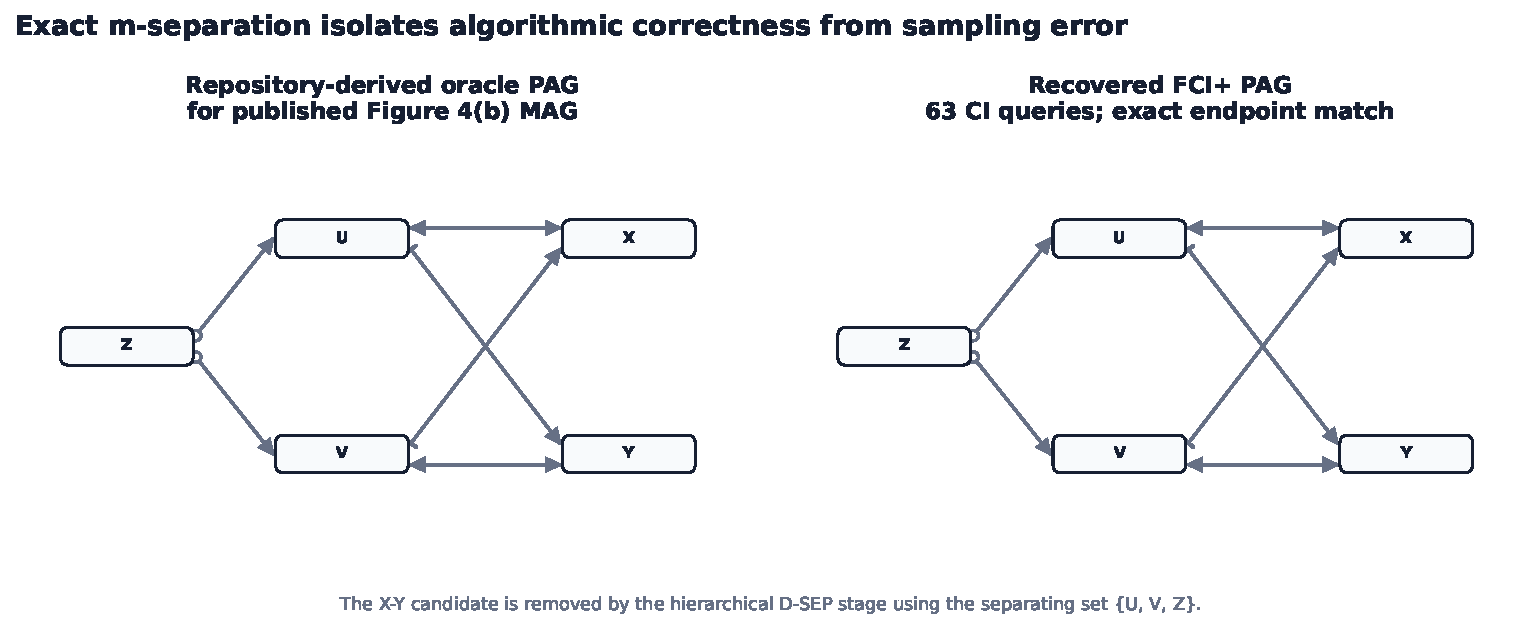
\includegraphics[width=\textwidth]{figure4_validation.pdf}
\caption{Exact-oracle validation on the central Figure 4(b) example. The
learned \FCIplus{} PAG matches every oracle adjacency and endpoint.}
\label{fig:figure4-validation}
\end{figure}

The initial adjacency stage retains the \(X-Y\) link. \FCIplus{} identifies it
as a D-SEP candidate and removes it using \(\{U,V,Z\}\). Standard FCI reaches
the same final PAG through Possible-D-SEP. The measured query counts on this
fixture are:

\begin{table}[H]
\centering
\caption{Paper-aligned Figure 4(b) oracle comparison.}
\label{tab:figure4-results}
\begin{tabular}{lrrl}
\toprule
Algorithm & CI queries & Difference & Final PAG \\
\midrule
Standard FCI & 102 & reference & Exact \\
\FCIplus{} & 63 & \(-39\) (\(-38.2\%\)) & Exact \\
\bottomrule
\end{tabular}
\end{table}

\section{Finite-sample integration test}

Exact CI answers are necessary for testing the algorithm, but real data
replace them with noisy statistical decisions. A seeded latent linear SEM
based on the same reference graph provides the following integration result:

\begin{table}[H]
\centering
\caption{Seeded finite-sample recovery on the Figure 4(b) SEM.}
\label{tab:finite-sample}
\begin{tabularx}{\textwidth}{p{0.16\textwidth}p{0.32\textwidth}p{0.26\textwidth}Y}
\toprule
Sample size & \FCIplus{} & Standard FCI & Interpretation \\
\midrule
\(N=5{,}000\) & Extra \(X\leftrightarrow Y\); exact F1 \(=0.923\) &
Exact PAG; exact F1 \(=1.000\) &
The sample CI decisions do not expose the \FCIplus{} D-SEP candidate. \\
\(N=50{,}000\) & Exact PAG; exact F1 \(=1.000\) &
Exact PAG; exact F1 \(=1.000\) &
Both algorithms recover this seeded fixture; this is not a universal sample
threshold. \\
\bottomrule
\end{tabularx}
\end{table}

This result is a useful warning against claiming that fewer CI tests imply
uniformly better finite-sample accuracy. FCI and \FCIplus{} can make different
errors because they use different logical search routes after the initial
skeleton.

\section{Reference software}

The STAR analysis runs CRAN \code{pcalg} 2.7-12 under R 4.5.3 as an independent
reference implementation \citep{kalisch2012pcalg}. The runner calls
\code{pcalg::fciPlus} with selection-bias orientations enabled. It supplies a
custom G-square test that exactly mirrors the Python compact-table rule:
zero-marginal rows and columns are removed separately within each observed
conditioning stratum, and the resulting likelihood-ratio statistics and
degrees of freedom are summed. This avoids \code{disCItest}'s default
minimum-cell shortcut, which would otherwise change the CI decisions rather
than merely change the implementation.

The R output is treated as a differential reference, not ground truth. In
particular, \code{pcalg::fciPlus} does not expose the local implementation's
explicit \(k=3\) sparsity-bound parameter. Comparisons therefore report
skeleton overlap, exact endpoint agreement, target-edge marks, runtime, CI
calls, and cyclic-order sensitivity instead of awarding correctness by package
name.

\medskip
\keyresult{The oracle tests support the correctness of the implemented FCI and
\FCIplus{} search-and-orientation pipeline under exact conditional-independence
information. The finite-sample tests simultaneously show that empirical
results remain limited by CI-test error and tuning choices.}

\part{Tennessee STAR Application}

\chapter{Study Design and Data}

\section{The Tennessee STAR experiment}

The Tennessee Student/Teacher Achievement Ratio project was a large
randomized experiment conducted in kindergarten through grade 3. Students and
teachers were assigned to small classes, regular classes, or regular classes
with a full-time aide. The official technical report describes small classes
of approximately 13--17 students and regular classes of approximately 22--25
students \citep{word1990star}. Subsequent economic analysis has used STAR as a
central source of evidence on class size and educational production
\citep{krueger1999experimental}.

The present analysis uses the official Harvard Dataverse release
\citep{achilles2008star}. The student-level file contains 11,601 records and
379 variables and is released under CC0 1.0. Data codes were checked against
the accompanying 146-page user guide.

\section{Why use causal discovery on a randomized experiment?}

Randomization already provides a stronger basis for estimating the class-size
effect than an unconstrained structure-learning algorithm. The purpose of FCI
is therefore not to rediscover or replace randomization. It is to examine:

\begin{itemize}[leftmargin=2em]
  \item whether grade-3 observation is structurally related to early
        achievement or background variables;
  \item whether early and later achievement remain adjacent after conditioning
        on the measured context;
  \item how the learned PAG changes when an early post-assignment outcome is
        included or excluded;
  \item whether FCI and \FCIplus{} agree on skeletons and important
        adjacencies;
  \item how much search work \FCIplus{} saves on a real dataset.
\end{itemize}

This design also provides an unusually useful external audit. If a data-only
PAG implies an implausible pre-treatment direction or suggests latent
confounding of a genuinely randomized assignment, the discrepancy should be
reported rather than accepted literally.

\section{Cohort construction}

The analysis begins with 6,325 students who have a kindergarten STAR class
assignment, representing 79 kindergarten schools. Three panels are constructed
for different questions.

\begin{table}[H]
\centering
\caption{STAR analysis panels.}
\label{tab:panels}
\begin{tabularx}{\textwidth}{p{0.22\textwidth}rrY}
\toprule
Panel & Rows & Nodes & Purpose \\
\midrule
Attrition / observation & 5,744 & 9 &
Relate kindergarten assignment, characteristics, context, and achievement to
whether both grade-3 reading and mathematics scores are observed. \\
Longitudinal achievement & 2,787 & 9 &
Study structure between kindergarten and grade-3 achievement among complete
cases while retaining early achievement. \\
Focused treatment-outcome & 2,976 & 8 &
Study the class-assignment/grade-3 relationship without allowing
kindergarten achievement, an early post-assignment outcome, to serve as a
separator. \\
\bottomrule
\end{tabularx}
\end{table}

The panels are intentionally not pooled. Each encodes a different statistical
question, and including or excluding kindergarten achievement changes the
meaning of separation between assignment and the later outcome.

\section{Variable coding}

\begin{longtable}{p{0.23\textwidth}p{0.23\textwidth}p{0.46\textwidth}}
\caption{Variables supplied to FCI and \FCIplus{}.}
\label{tab:variables}\\
\toprule
Analysis variable & Source fields & Coding \\
\midrule
\endfirsthead
\toprule
Analysis variable & Source fields & Coding \\
\midrule
\endhead
\code{K\_Class} & \code{gkclasstype} &
Small, regular, or regular with aide. \\
\code{Gender} & \code{gender} &
Male or female, using the official data codes. \\
\code{Ethnicity} & \code{race} &
White, Black, or Other; smaller source categories are collapsed to avoid
extremely sparse contingency cells. \\
\code{Free\_Lunch} & \code{gkfreelunch} &
Free/reduced-price lunch versus non-free lunch. \\
\code{School\_Context} & \code{gksurban} &
Inner city, suburban, rural, or urban. \\
\code{Entry\_Age} & \code{birthyear}, \code{birthmonth} &
Age in months at September 1985, converted to four quantile categories. \\
\code{Teacher\_Experience} & \code{gktyears} &
0--5, 6--10, 11--20, or 21+ years. \\
\code{K\_Achievement} & \code{gktreadss}, \code{gktmathss} &
Reading plus mathematics scaled score, converted to kindergarten achievement
quartiles. \\
\code{Grade3\_Achievement} & \code{g3treadss}, \code{g3tmathss} &
Reading plus mathematics scaled score, converted to grade-3 achievement
quartiles among students with both scores. \\
\code{Grade3\_Observed} & \code{g3treadss}, \code{g3tmathss} &
Indicator that both grade-3 scores are present. \\
\bottomrule
\end{longtable}

All model inputs are integer-coded discrete categories. The exact numeric
tables supplied to the algorithms are committed under
\path{case_studies/tennessee_star/data/processed}.

\chapter{STAR Analysis Methods}

\section{Descriptive randomized-arm reference}

Before causal discovery, the report computes observed means and
randomized-arm contrasts for:

\begin{enumerate}[leftmargin=2em]
  \item the sum of kindergarten reading and mathematics scaled scores;
  \item the sum of grade-3 reading and mathematics scaled scores among
        students with both scores;
  \item the probability that both grade-3 scores are observed.
\end{enumerate}

Uncertainty is estimated with 1,000 bootstrap samples of kindergarten schools.
Resampling schools rather than individual students preserves the main
within-school dependence in the descriptive comparison. These contrasts are
reported separately from FCI output because they use the experiment's
assignment as the basis for interpretation.

\section{Discrete G-square conditional-independence test}

The application uses the likelihood-ratio G-square test. For variables \(X\)
and \(Y\), conditioning set \(S\), observed contingency counts \(O\), and
expected counts \(E\) under \(X\perp Y\mid S\), the statistic is
\[
  G^2 = 2\sum_{s}\sum_{x,y}
        O_{xys}\log\left(\frac{O_{xys}}{E_{xys}}\right),
\]
with zero-count contributions omitted. The test is appropriate for the
discretised panels, but high-order conditioning can create sparse cells. That
is one reason the \FCIplus{} bound is fixed at \(k=3\) and why sensitivity is
reported rather than hidden.

\section{Primary discovery configuration}

\begin{table}[H]
\centering
\caption{Primary STAR discovery configuration.}
\label{tab:star-config}
\begin{tabularx}{\textwidth}{p{0.30\textwidth}Y}
\toprule
Setting & Value \\
\midrule
CI test & G-square on discretised variables \\
Significance threshold & \(\alpha=0.05\) \\
Standard FCI & \code{profile="paper"}; unbounded paper schedule \\
\FCIplus{} & \code{profile="paper"}; \(k=3\) \\
R reference & \code{pcalg::fciPlus}; selection bias enabled; no exposed
explicit \(k\) setting \\
Timing & Three full-data repetitions; median elapsed time reported \\
PAG stability & 12 kindergarten-school cluster bootstrap fits per algorithm
and panel for the two self-implemented algorithms \\
Random seed & Fixed by the application script for reproducibility \\
Prior temporal constraints & None supplied to discovery; temporal reversals
are audited after fitting \\
\bottomrule
\end{tabularx}
\end{table}

Not imposing temporal or randomization constraints allows the analysis to test
the behaviour of the data-only algorithm. It also means that implausible
orientations must not be treated as credible causal chronology.

\section{School-cluster PAG stability}

For each panel and algorithm, the 79 kindergarten schools are sampled with
replacement. All student rows from a selected school are included, including
repeated copies when a school is sampled more than once. FCI or \FCIplus{} is
then refitted and the presence of each unordered adjacency is recorded.

With \(B=12\) replicates, the estimated adjacency frequency is
\[
  \widehat{\pi}_{XY}
  = \frac{1}{B}\sum_{b=1}^{B}
    \mathbf{1}\{X\text{ and }Y\text{ are adjacent in replicate }b\}.
\]
This is an exploratory stability diagnostic. Twelve replicates give a coarse
grid of 8.3 percentage points and are not sufficient for precise tail
probabilities.

\section{Sensitivity analysis}

\enlargethispage{3\baselineskip}

The focused treatment-outcome analysis is repeated for:

\begin{itemize}[leftmargin=2em]
  \item \(\alpha\in\{0.01,0.05\}\);
  \item three versus four quantile bins for age and achievement;
  \item standard FCI and \FCIplus{}.
\end{itemize}

The target is whether \code{K\_Class} remains adjacent to
\code{Grade3\_Achievement}. This directly tests whether the most
substantively tempting PAG edge is robust to reasonable analysis choices.

\chapter{STAR Results}

\section{Observed randomized-arm outcomes}

\begin{table}[H]
\centering
\caption{Observed outcome summaries by kindergarten class arm. Intervals use
1,000 kindergarten-school bootstrap samples.}
\label{tab:arm-summary}
\begin{threeparttable}
\begin{tabular}{llrrr}
\toprule
Outcome & Arm & \(n\) & Estimate & 95\% interval \\
\midrule
\multirow{3}{*}{Kindergarten score}
 & Regular & 2,005 & 918.04 & 908.78 to 927.05 \\
 & Regular + aide & 2,043 & 918.36 & 908.52 to 927.07 \\
 & Small & 1,738 & 931.94 & 922.70 to 940.12 \\
\addlinespace
\multirow{3}{*}{Grade-3 score}
 & Regular & 1,047 & 1246.74 & 1238.96 to 1254.01 \\
 & Regular + aide & 1,019 & 1247.25 & 1238.53 to 1255.48 \\
 & Small & 936 & 1258.43 & 1250.58 to 1266.17 \\
\addlinespace
\multirow{3}{*}{Grade-3 observed}
 & Regular & 2,194 & 47.72\% & 42.72\% to 52.14\% \\
 & Regular + aide & 2,231 & 45.67\% & 40.64\% to 50.39\% \\
 & Small & 1,900 & 49.26\% & 44.46\% to 53.77\% \\
\bottomrule
\end{tabular}
\begin{tablenotes}[flushleft]\small
\item Grade-3 score summaries condition on both reading and mathematics scores
being observed. Kindergarten score summaries also exclude missing score
components, so they are design-supported observed-outcome comparisons rather
than a fully reconstructed intention-to-treat estimand.
\end{tablenotes}
\end{threeparttable}
\end{table}

\begin{figure}[H]
\centering
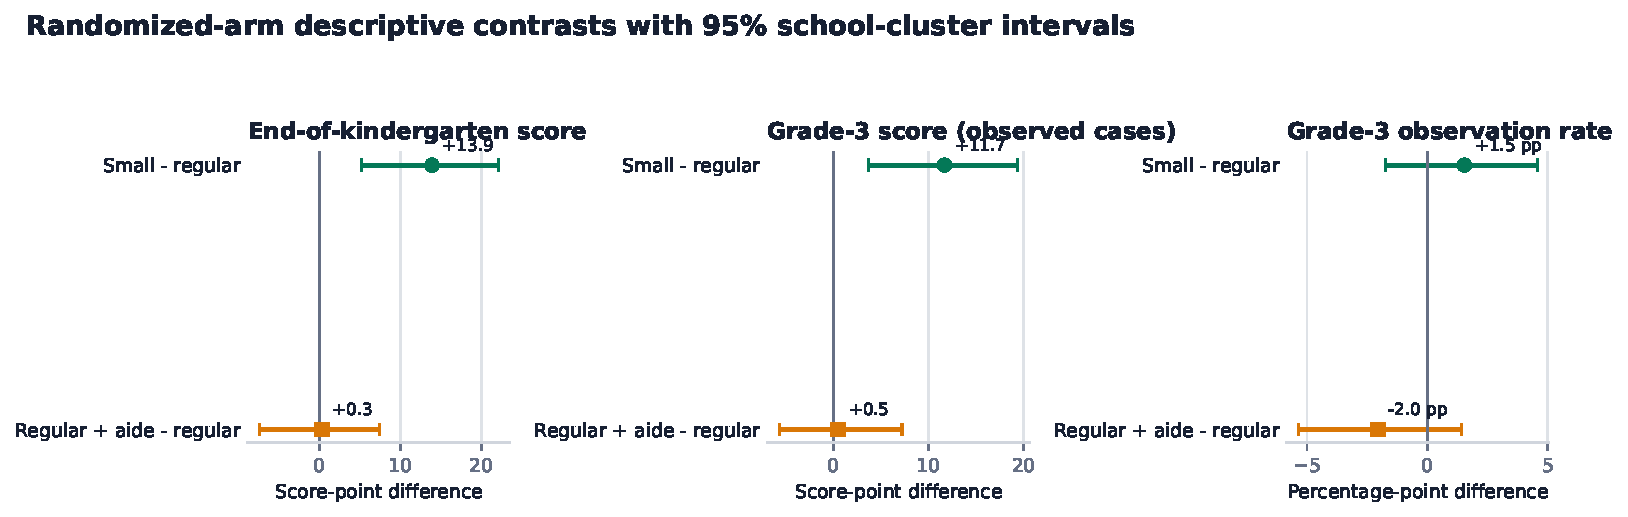
\includegraphics[width=\textwidth]{star_descriptive_contrasts.pdf}
\caption{Contrasts against the regular-class arm. Small classes show positive
score differences at kindergarten and grade 3 among observed cases; the aide
arm remains close to zero.}
\label{fig:descriptive-contrasts}
\end{figure}

The small-minus-regular kindergarten contrast is \(13.90\) points, with a 95\%
school-cluster interval from \(5.21\) to \(22.07\). The regular-with-aide
contrast is \(0.31\) points, with an interval from \(-7.40\) to \(7.38\).

At grade 3 among observed students, the small-class contrast remains positive
at \(11.69\) points (3.74 to 19.38). The aide contrast is \(0.51\) points
(\(-5.70\) to \(7.22\)). Observation rates themselves do not show a precise
class-arm difference: small minus regular is \(+1.54\) percentage points
(\(-1.73\) to \(4.56\)), while aide minus regular is \(-2.05\) points
(\(-5.35\) to \(1.41\)).

\keyresult{The observed randomized-arm evidence supports a small-class
achievement advantage and does not support a comparable advantage from adding
an aide to a regular class. The grade-3 score contrast is conditional on later
observation and therefore has a weaker causal interpretation than the early
outcome comparison.}

\section{Attrition and grade-3 observation}

\begin{figure}[H]
\centering
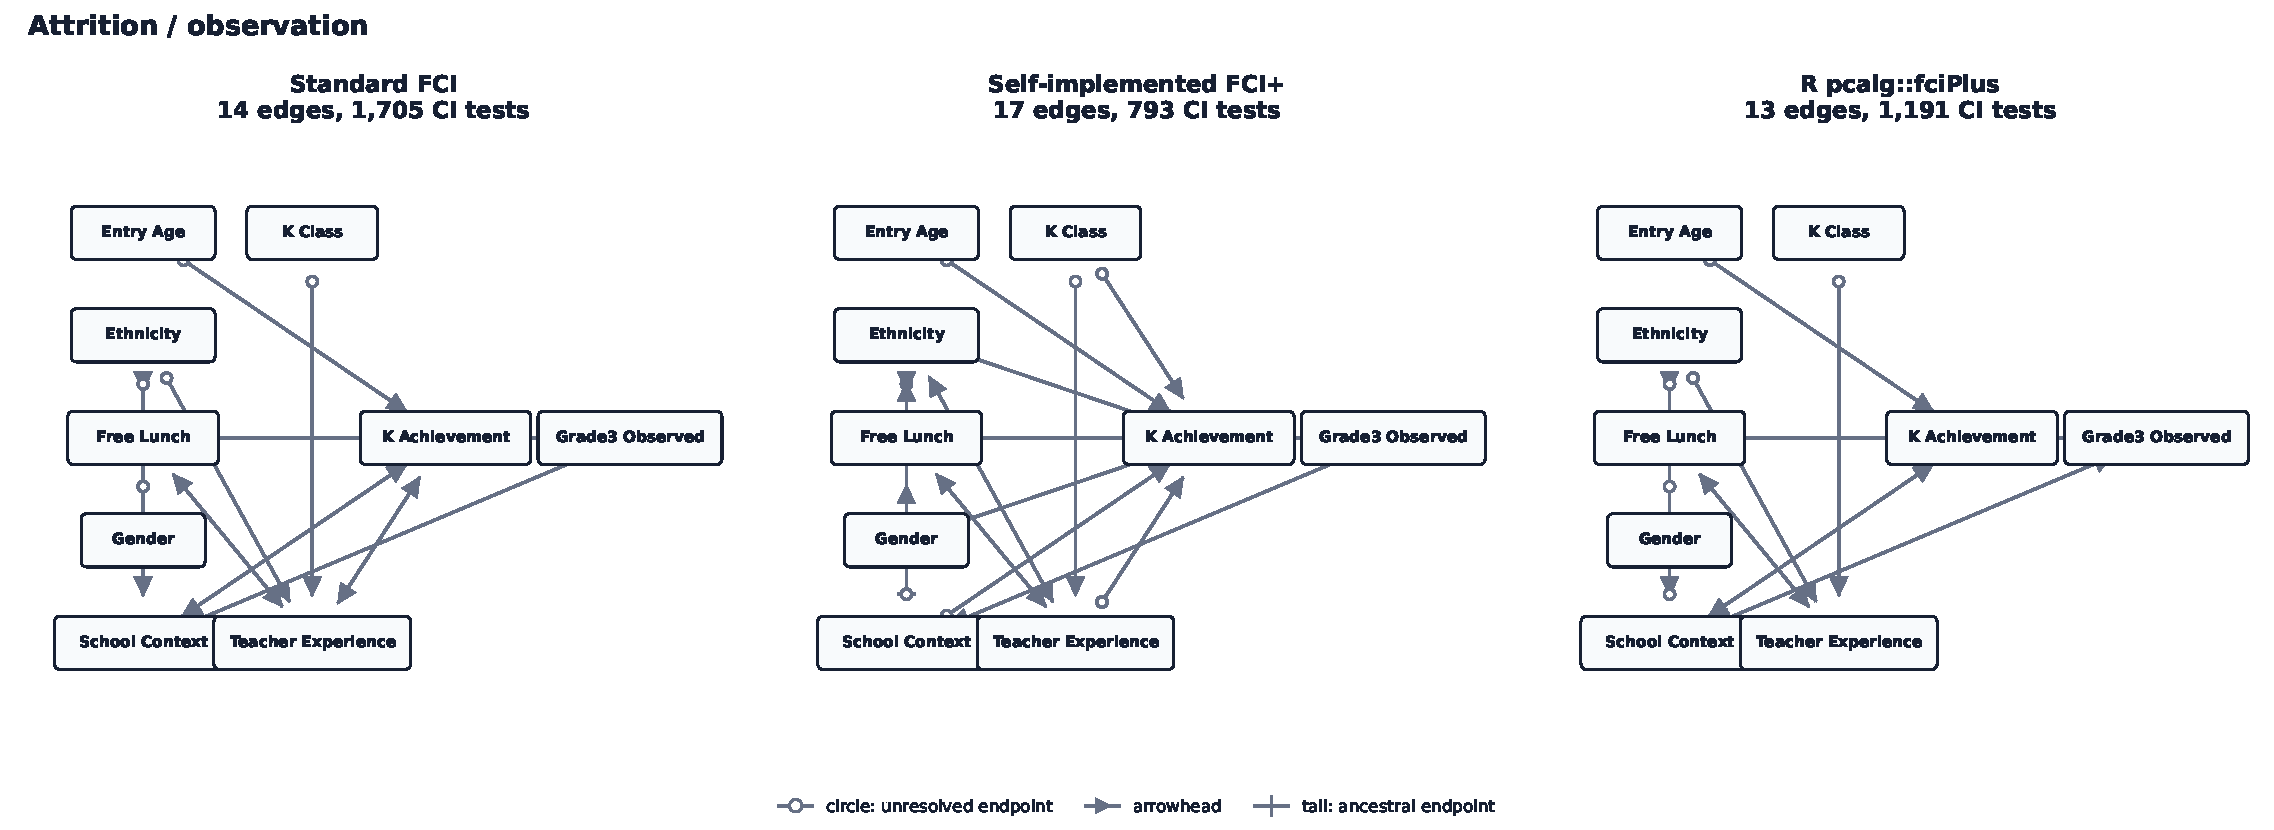
\includegraphics[width=\textwidth]{pag_attrition.pdf}
\caption{Three PAGs for the attrition/observation panel: self-implemented FCI,
self-implemented \FCIplus{}, and R \code{pcalg::fciPlus}. The skeletons
substantially overlap, while the achievement/observation endpoint differs.}
\label{fig:pag-attrition}
\end{figure}

Standard FCI returns 14 edges after 1,705 CI tests; self-implemented
\FCIplus{} returns 17 edges after 793 tests; and R \code{pcalg::fciPlus}
returns 13 edges after 1,191 tests. The FCI/self-\FCIplus{},
FCI/R-\FCIplus{}, and self-/R-\FCIplus{} skeleton Jaccard values are 0.824,
0.929, and 0.765. All three omit a direct
\code{K\_Class}--\code{Grade3\_Observed} adjacency. In the self-implementation
school bootstrap that adjacency appears in only 17\% of FCI fits and 8\% of
\FCIplus{} fits.

By contrast, \code{K\_Achievement}--
\code{Grade3\_Observed} is adjacent in 100\% of the bootstrap fits for both
algorithms. The corresponding free-lunch/observation adjacency is also stable
in the targeted audit. These results suggest that later data availability is
not independent of early achievement and measured socioeconomic or school
context.

The three endpoint readings are revealing. Standard FCI gives the impossible
\textit{grade-3 observation} \(\rightarrow\) \textit{kindergarten
achievement}; self-\FCIplus{} leaves a circle at the later endpoint; and
R-\FCIplus{} gives the temporally admissible
\textit{kindergarten achievement} \(\rightarrow\) \textit{grade-3
observation}. The R result is more plausible on this edge, but package identity
alone cannot establish that its orientation is statistically correct.

\cautionbox{The attrition PAG does not prove a particular missingness
mechanism. It shows that the observed conditional-independence structure links
grade-3 availability to earlier achievement and context. A formal
missing-data analysis would require an explicit estimand and additional
assumptions.}

\section{Longitudinal achievement}

\begin{figure}[H]
\centering
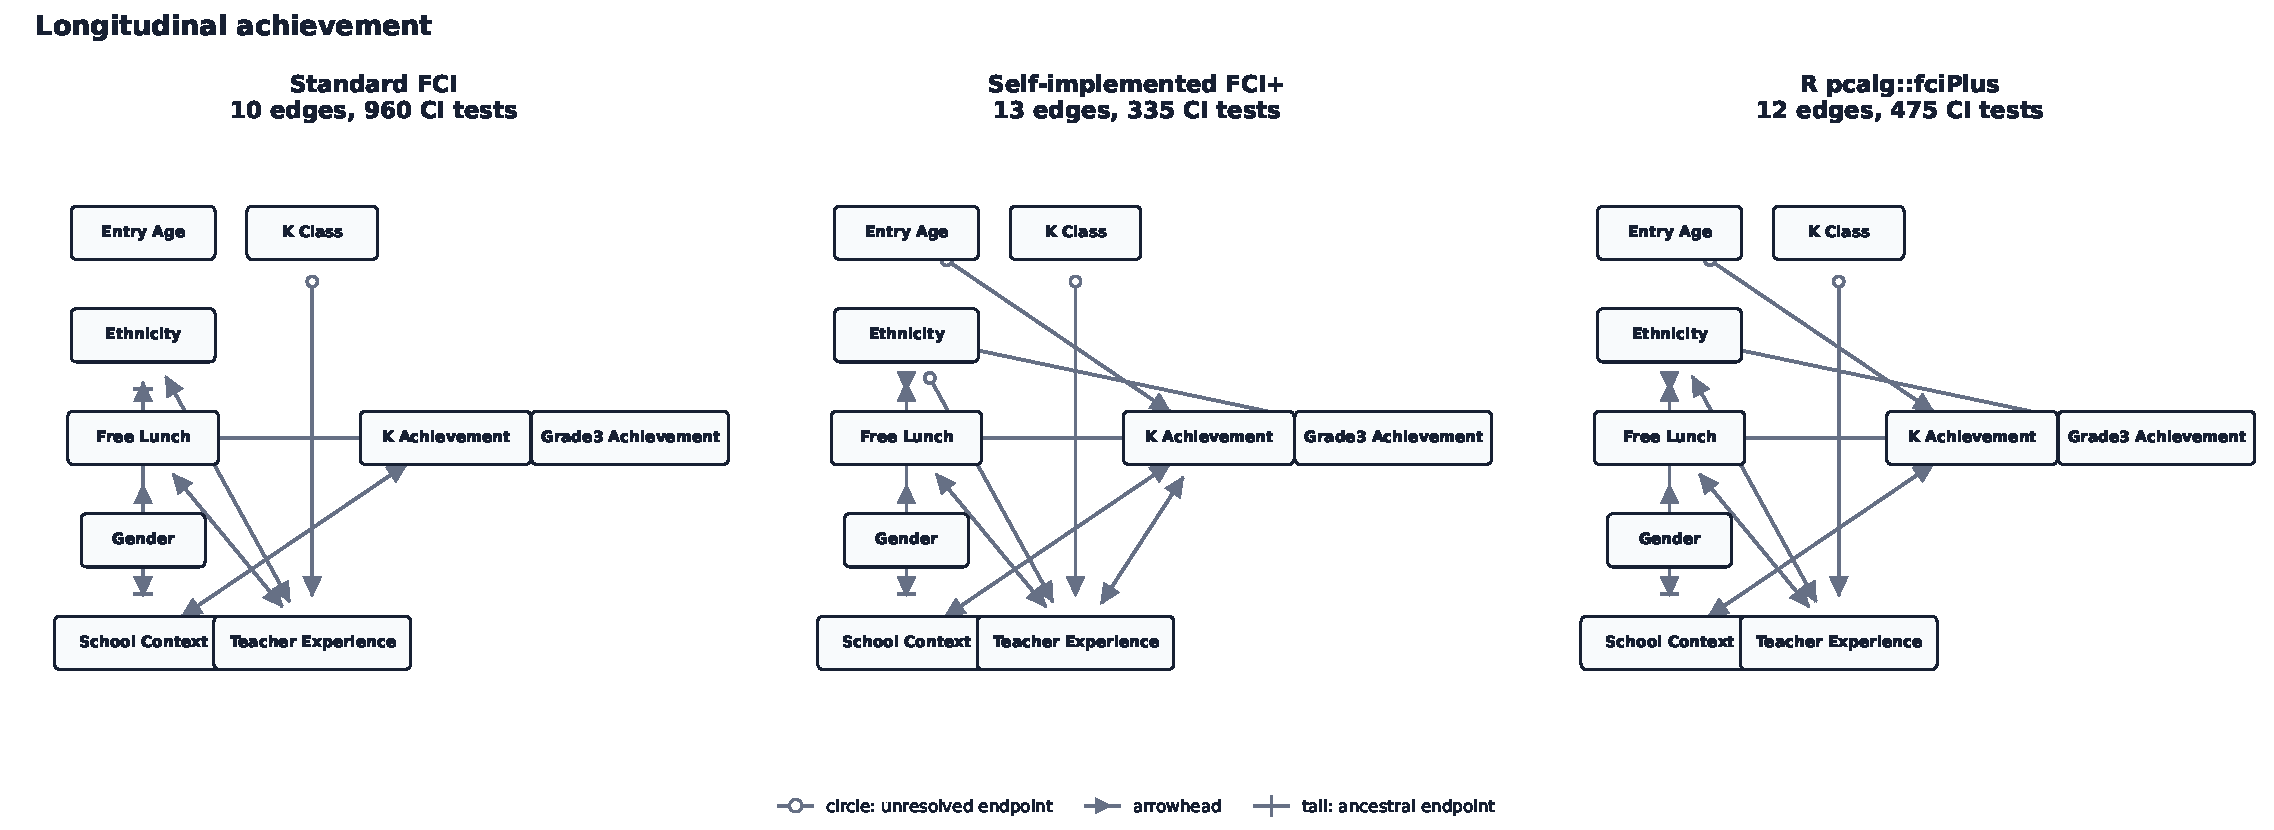
\includegraphics[width=\textwidth]{pag_longitudinal.pdf}
\caption{Three PAGs for the longitudinal complete-case panel. All retain the
kindergarten/grade-3 achievement adjacency, but the two \FCIplus{}
implementations orient it against chronology.}
\label{fig:pag-longitudinal}
\end{figure}

Standard FCI returns 10 edges and 960 CI tests. Self-\FCIplus{} returns 13
edges and 335 tests, while R-\FCIplus{} returns 12 edges and 475 tests.
Pairwise skeleton Jaccard is 0.769 for FCI/self-\FCIplus{}, 0.833 for FCI/R,
and 0.923 for the two \FCIplus{} implementations.

All three algorithms retain the kindergarten/grade-3 achievement adjacency,
and it appears in all 12 school-cluster bootstrap samples for both local
algorithms.
Neither full-data PAG retains a direct class-assignment/grade-3 achievement
adjacency once kindergarten achievement is included. That treatment-outcome
adjacency nevertheless reappears in 50\% of FCI and 67\% of \FCIplus{}
bootstrap fits, indicating moderate instability across resampled schools.

Both \FCIplus{} implementations orient grade-3 achievement toward
kindergarten achievement, which is temporally impossible if read causally.
Standard FCI leaves the grade-3 endpoint unresolved. The agreement between two
implementations is therefore not sufficient to override chronology: it may
replicate the same finite-sample CI pattern and orientation logic under
complete-case selection.

\section{Focused treatment-outcome panel}

\begin{figure}[H]
\centering
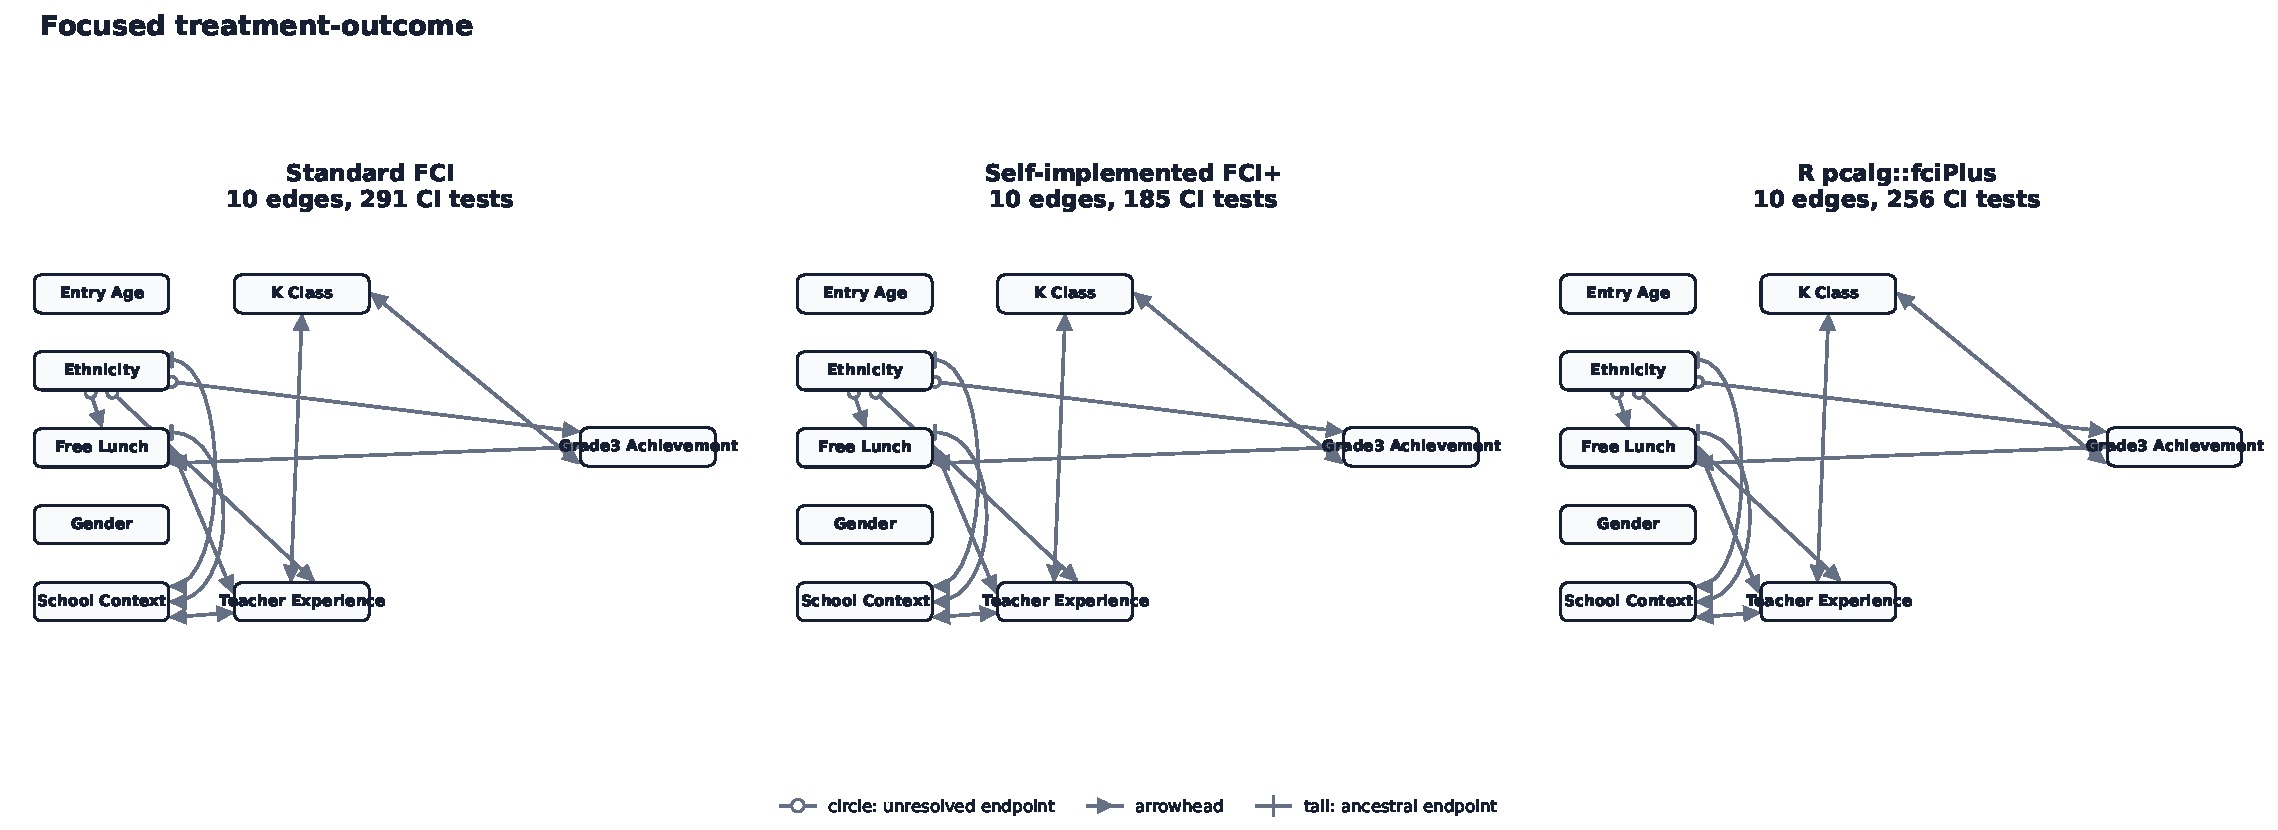
\includegraphics[width=\textwidth]{pag_focused_treatment.pdf}
\caption{PAGs for the focused complete-case panel. All three algorithms recover
the exact same 10-edge skeleton and endpoint pattern, including the bidirected
class-assignment/grade-3 edge.}
\label{fig:pag-focused}
\end{figure}

Removing kindergarten achievement from the node set changes the result.
Standard FCI, self-\FCIplus{}, and R-\FCIplus{} all return the same 10-edge
PAG, not merely the same skeleton. All three contain
\[
  K\_\mathrm{Class}\leftrightarrow
  Grade3\_\mathrm{Achievement}.
\]
The adjacency appears in 92\% of the FCI school bootstraps and 83\% of the
self-\FCIplus{} bootstraps. The independent exact PAG replication makes this
observed conditional-independence pattern more credible, but does not make the
literal latent-confounding interpretation credible.

A naive reading would call the bidirected edge evidence of latent confounding.
That reading is not defensible here. Kindergarten class assignment was
randomized, while the focused panel conditions on grade-3 outcomes being
observed and omits early post-assignment achievement. Conditioning on
observation, school-level dependence, omitted post-randomization variables,
and CI-test approximation can all create an observed independence pattern
that is represented by arrowheads at both endpoints.

\section{Stability and sensitivity}

\begin{figure}[H]
\centering
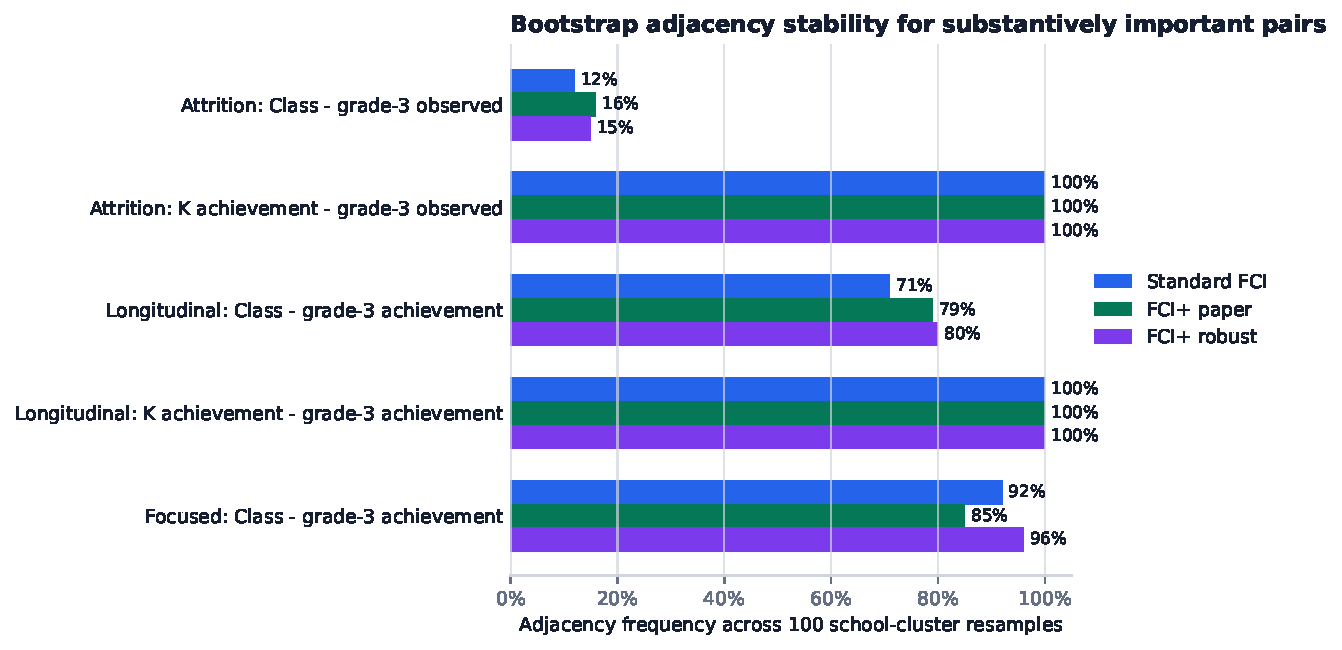
\includegraphics[width=\textwidth]{star_bootstrap_stability.pdf}
\caption{School-cluster adjacency frequencies for selected pairs. Frequencies
measure skeleton stability only; they do not validate endpoint orientation.}
\label{fig:bootstrap-stability}
\end{figure}

\begin{figure}[H]
\centering
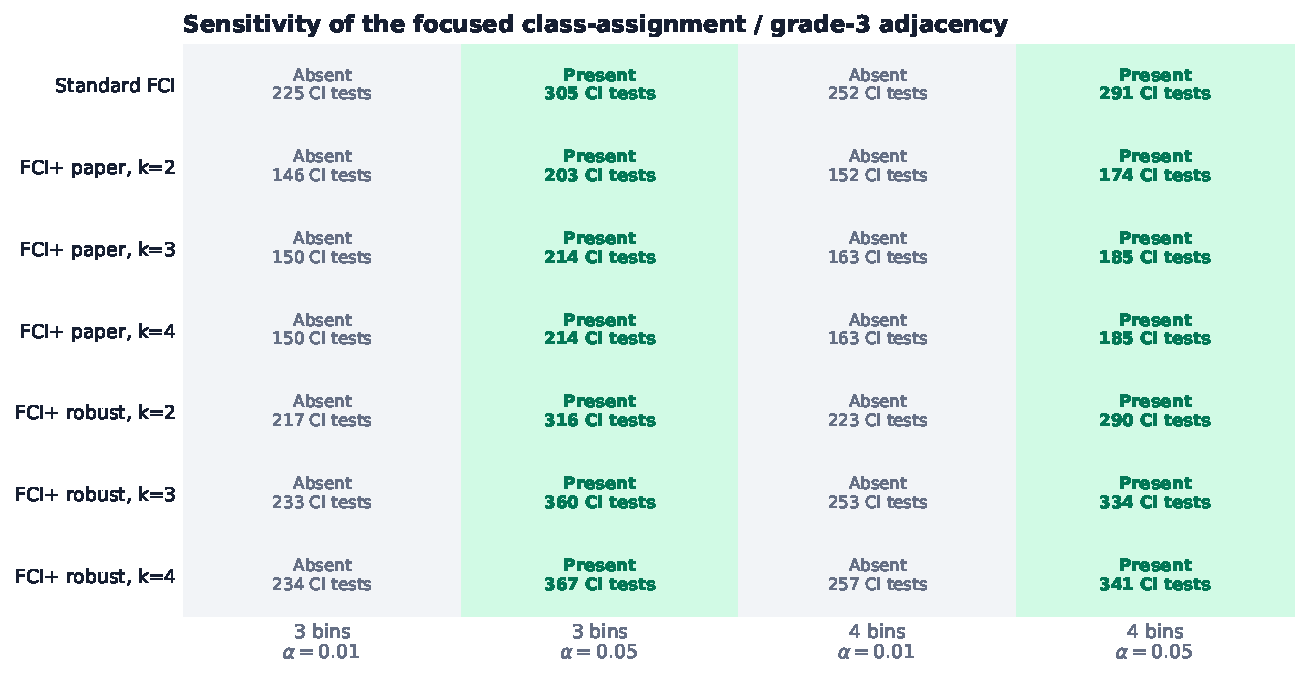
\includegraphics[width=0.92\textwidth]{star_sensitivity.pdf}
\caption{Focused treatment-outcome sensitivity. The adjacency appears at
\(\alpha=0.05\) and disappears at \(\alpha=0.01\), regardless of whether three
or four quantile bins are used.}
\label{fig:sensitivity}
\end{figure}

The sensitivity result is decisive for interpretation. The focused
treatment-outcome adjacency is robust to the tested bin count but not to the
CI threshold. At \(\alpha=0.01\), neither algorithm retains it; at
\(\alpha=0.05\), both retain the same bidirected mark.

The stronger threshold requires more evidence against conditional
independence before an edge is kept. Its removal therefore indicates that the
edge is driven by relatively weak conditional-dependence evidence, not an
invariant feature across reasonable test settings.

\section{Cross-implementation agreement and order audit}

\begin{figure}[H]
\centering
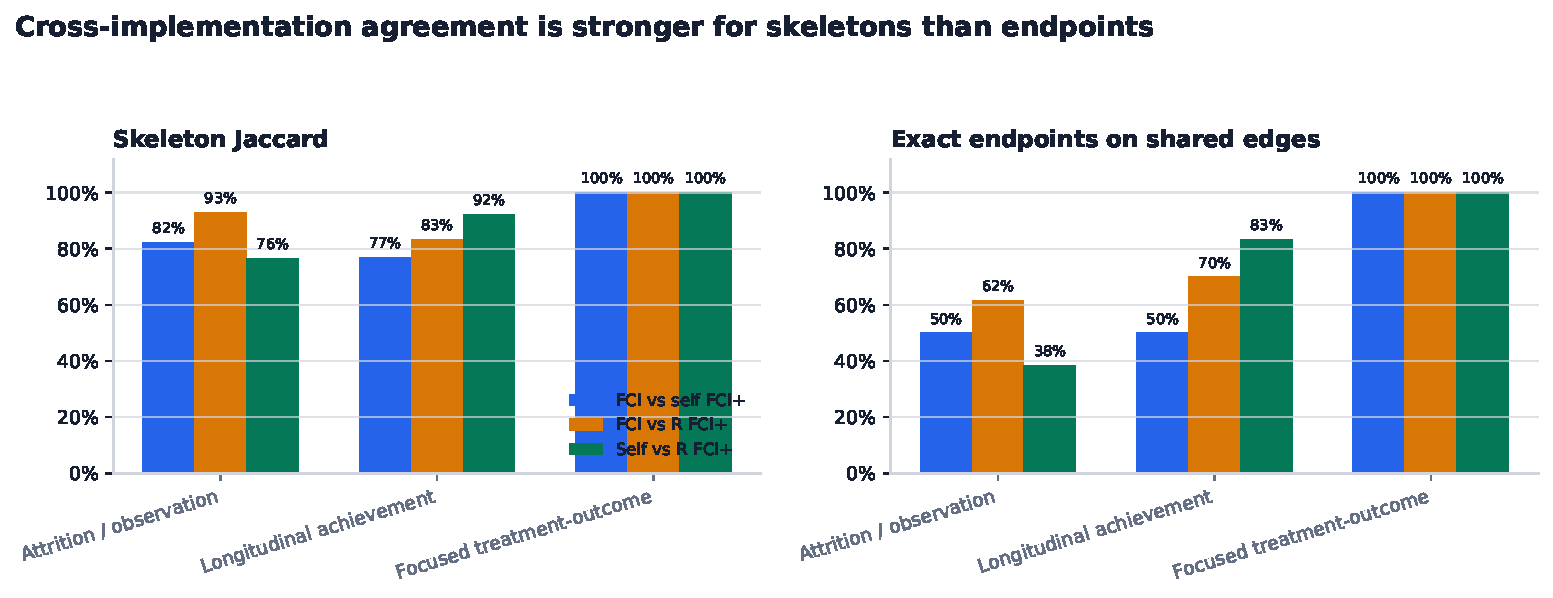
\includegraphics[width=\textwidth]{star_three_algorithm_agreement.pdf}
\caption{Pairwise skeleton Jaccard and exact endpoint agreement on shared
edges. Skeleton agreement is consistently stronger than endpoint agreement
outside the focused panel.}
\label{fig:three-algorithm-agreement}
\end{figure}

\begin{table}[H]
\centering
\caption{Three-algorithm structural agreement. Endpoint rates use only
adjacencies shared by the indicated pair.}
\label{tab:three-algorithm-agreement}
\begin{tabular}{llrr}
\toprule
Panel & Pair & Skeleton Jaccard & Exact endpoint rate \\
\midrule
\multirow{3}{*}{Attrition}
 & FCI / self-\FCIplus{} & 0.824 & 50.0\% \\
 & FCI / R-\FCIplus{} & 0.929 & 61.5\% \\
 & self- / R-\FCIplus{} & 0.765 & 38.5\% \\
\addlinespace
\multirow{3}{*}{Longitudinal}
 & FCI / self-\FCIplus{} & 0.769 & 50.0\% \\
 & FCI / R-\FCIplus{} & 0.833 & 70.0\% \\
 & self- / R-\FCIplus{} & 0.923 & 83.3\% \\
\addlinespace
\multirow{3}{*}{Focused}
 & FCI / self-\FCIplus{} & 1.000 & 100.0\% \\
 & FCI / R-\FCIplus{} & 1.000 & 100.0\% \\
 & self- / R-\FCIplus{} & 1.000 & 100.0\% \\
\bottomrule
\end{tabular}
\end{table}

\begin{figure}[H]
\centering
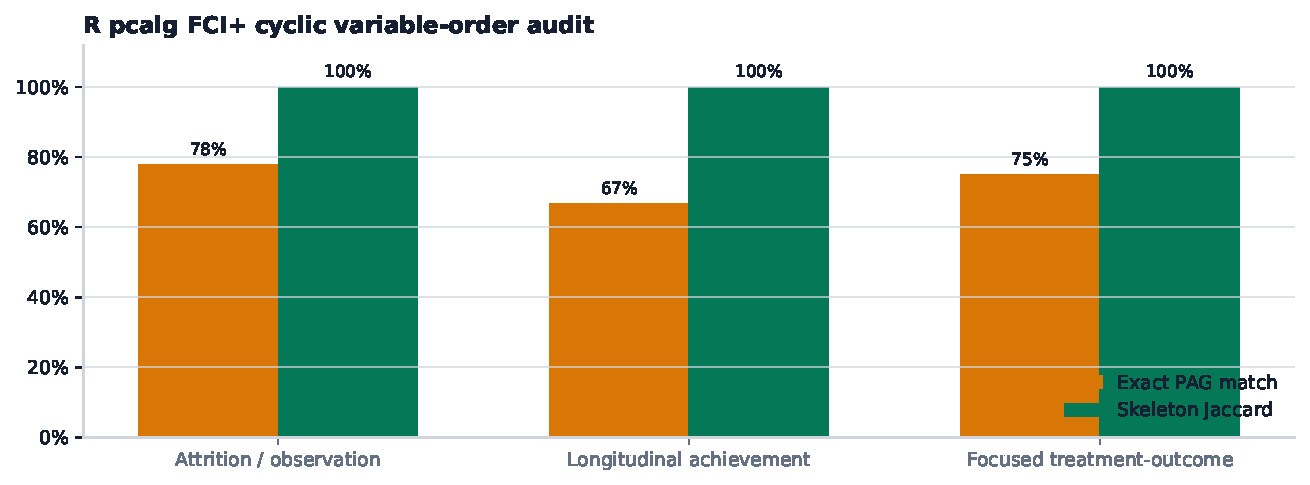
\includegraphics[width=0.94\textwidth]{star_pcalg_order_audit.pdf}
\caption{R \code{pcalg::fciPlus} cyclic-order audit. Every tested order
reproduces the original skeleton, whereas exact endpoint reproduction ranges
from 67\% to 78\% across panels.}
\label{fig:pcalg-order-audit}
\end{figure}

The order audit rotates the input variable list through every cyclic shift.
All 26 refits preserve their panel's skeleton exactly. Exact PAG endpoints are
reproduced in 7 of 9 attrition orders, 6 of 9 longitudinal orders, and 6 of 8
focused orders. Thus the R reference strongly supports skeleton robustness in
this audit, but also independently demonstrates that some endpoint marks are
implementation-order sensitive.

\section{Computational comparison}

\begin{figure}[H]
\centering
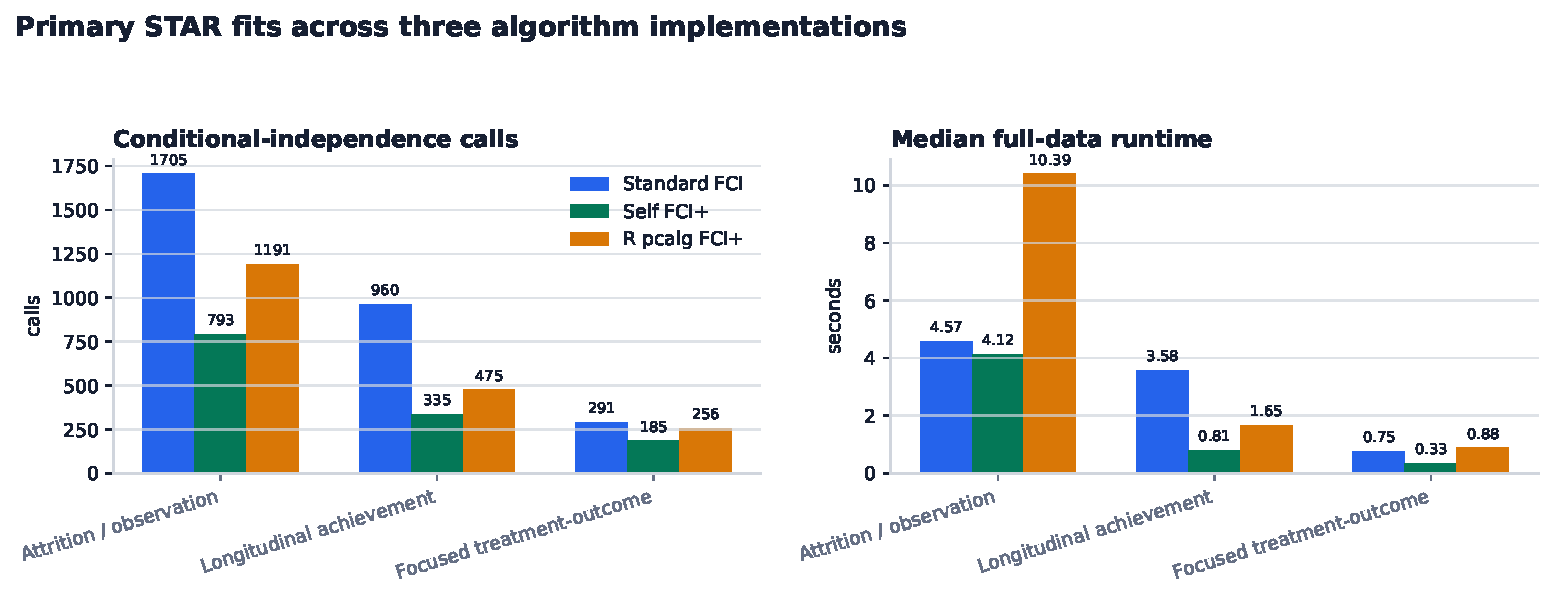
\includegraphics[width=\textwidth]{star_performance.pdf}
\caption{Full-data search work and median runtime. All algorithms use the same
panel, compact-table G-square test, and \(\alpha=0.05\); internal search
schedules and language runtimes are not identical.}
\label{fig:performance}
\end{figure}

\begin{table}[H]
\centering
\caption{Three-algorithm performance on the STAR panels.}
\label{tab:performance}
\begin{tabular}{llrrr}
\toprule
Panel & Algorithm & Edges & CI tests & Median seconds \\
\midrule
\multirow{3}{*}{Attrition}
 & FCI & 14 & 1,705 & 4.568 \\
 & Self-\FCIplus{} & 17 & 793 & 4.118 \\
 & R-\FCIplus{} & 13 & 1,191 & 10.394 \\
\addlinespace
\multirow{3}{*}{Longitudinal}
 & FCI & 10 & 960 & 3.577 \\
 & Self-\FCIplus{} & 13 & 335 & 0.805 \\
 & R-\FCIplus{} & 12 & 475 & 1.650 \\
\addlinespace
\multirow{3}{*}{Focused}
 & FCI & 10 & 291 & 0.754 \\
 & Self-\FCIplus{} & 10 & 185 & 0.330 \\
 & R-\FCIplus{} & 10 & 256 & 0.884 \\
\bottomrule
\end{tabular}
\end{table}

\FCIplus{} uses 46.5\%, 34.9\%, and 63.6\% of the standard FCI CI-test counts
on the attrition, longitudinal, and focused panels. The independent R
\FCIplus{} uses 69.9\%, 49.5\%, and 88.0\% of the corresponding standard-FCI
counts. Runtime is not a language-neutral benchmark: the R runner includes
R-level contingency-table construction, whereas the Python implementation
uses the package's native data path. CI-call counts are the more interpretable
search-work comparison.

These results demonstrate reduced search work, not universal algorithmic
dominance. In the two panels where skeleton Jaccard is below one, efficiency
and empirical structure differ simultaneously.

\chapter{Causal Interpretation}

\section{What can be concluded}

\subsection{Small classes improve early observed achievement}

STAR's random assignment is the primary causal identification mechanism.
Within the kindergarten cohort and among students with observed score
components, the small-class arm is 13.9 points above the regular arm, with a
school-cluster interval that excludes zero. This supports a beneficial causal
effect of smaller classes on early achievement, subject to outcome
missingness, assignment compliance, and the use of the observed composite
score.

The PAG is consistent with an assignment/achievement connection in the
\FCIplus{} attrition panel, but the causal conclusion does not depend on that
endpoint. It depends on the experiment.

\subsection{Adding an aide does not show the same advantage}

The regular-with-aide contrasts are close to zero at kindergarten and grade 3,
and both intervals include zero. In these observed data there is no evidence
that adding an aide to a regular-size class reproduces the achievement
advantage of reducing class size.

\subsection{Early achievement strongly predicts later structure}

Kindergarten and grade-3 achievement remain adjacent in the full longitudinal
fits of all three algorithms and in 100\% of the self-implementation school
bootstraps. Kindergarten achievement is also adjacent to grade-3 observation
in all three attrition fits. Cross-implementation agreement therefore supports
a robust \emph{skeleton-level} relationship between early performance, later
performance, and later data availability.

This finding still does not quantify mediation. Kindergarten achievement is a
post-assignment variable, and a formal mediation analysis would require
additional counterfactual assumptions. Moreover, the direction of the
longitudinal achievement edge fails the chronological audit for both
\FCIplus{} implementations.

\subsection{Attrition is selective but not clearly caused by class arm}

The full-data attrition PAGs do not retain a direct class-arm/observation
adjacency, and its bootstrap frequency is low. Observation is more stably
connected to early achievement and measured context. The evidence therefore
supports concern about selective attrition without showing a stable direct
effect of class arm on grade-3 observation.

\section{What cannot be concluded}

\begin{enumerate}[leftmargin=2em]
  \item \textbf{No unique DAG is identified.} Every PAG represents an
        equivalence class.
  \item \textbf{No causal effect magnitude comes from FCI.} The score
        differences are arm contrasts; PAG edges contain no ``points gained''
        coefficient.
  \item \textbf{A bidirected edge is not proof of a hidden confounder.} In the
        focused panel it conflicts with the known randomization unless
        selection, post-treatment conditioning, or other violations are
        considered.
  \item \textbf{The grade-3 contrast is not a complete long-run
        intention-to-treat estimate.} It conditions on observed grade-3
        outcomes.
  \item \textbf{Temporal reversals are not credible chronology.} They are
        algorithm diagnostics under violated or approximate assumptions.
  \item \textbf{Implementation agreement is not proof.} Shared CI decisions
        and shared logical rules can reproduce the same wrong endpoint.
\end{enumerate}

\keyresult{The strongest causal conclusion is design-based: smaller
kindergarten classes improve early observed achievement relative to regular
classes, while the aide arm shows no comparable effect. The main contribution
of the three-algorithm comparison is to separate replicated skeleton structure
from unstable endpoint orientation. It exposes selection, persistence, and
specification sensitivity around the experiment; it does not replace it.}

\chapter{Critical Self-Assessment}

\section{Strengths}

\begin{itemize}[leftmargin=2em]
  \item The algorithm and application are physically and logically separated.
  \item The data source, user guide, exact model inputs, random seeds, result
        tables, and report artifacts are committed.
  \item Standard FCI is always reported alongside \FCIplus{}.
  \item An independently maintained R implementation is run with matched CI
        semantics and its disagreements are retained in the report.
  \item Randomized-arm evidence is separated from exploratory PAG evidence.
  \item School-level resampling acknowledges the most important clustering
        unit.
  \item Endpoint reversals and threshold sensitivity are reported as failures
        of literal interpretation rather than silently corrected.
  \item The software is validated with exact oracle graphs, finite-sample
        integration tests, strict typing, multi-version tests, and wheel
        installation checks.
\end{itemize}

\section{Statistical limitations}

\subsection{Discretisation and sparse contingency tables}

Achievement and age are reduced to quantile categories, and teacher
experience is binned. This enables G-square testing across mixed educational
variables but discards within-bin information. As conditioning sets grow,
some multiway contingency cells may have small expected counts, weakening
the chi-square approximation.

\subsection{Dependence within schools and classrooms}

The primary CI test treats student rows as independent. The bootstrap
resamples schools, which measures sensitivity to school composition, but it
does not turn each underlying G-square test into a cluster-robust CI test.
Classroom identifiers and multilevel structure should be incorporated in a
more specialised analysis.

\subsection{Complete-case selection}

The longitudinal and focused panels require grade-3 scores. If observation is
affected by prior achievement, mobility, family circumstances, or school
processes, conditioning on complete cases may open selection paths. The
attrition panel provides evidence that observation is structurally related to
early variables, reinforcing this concern.

\subsection{Post-treatment variables}

Kindergarten achievement and teacher experience are measured during the
treatment period. They are not baseline covariates in the same sense as sex or
ethnicity. Including kindergarten achievement may block part of the
class-size pathway; excluding it may leave omitted post-treatment dependence.
The two panels deliberately show both specifications instead of selecting the
one with the preferred edge.

\subsection{Faithfulness and finite-sample CI error}

FCI-family guarantees rely on faithfulness and correct CI decisions. Near-zero
or cancelling effects may violate faithfulness, while finite samples produce
false dependence and false independence. The threshold-sensitive focused edge
is a direct example of this limitation.

\subsection{Unknown sparsity bound}

The \FCIplus{} paper profile uses \(k=3\). The true maximum degree of the
underlying STAR MAG is not observed and cannot be verified from the learned
graph alone. If the required separating set exceeds the bound, \FCIplus{} may
retain an extra edge. Conversely, \code{pcalg::fciPlus} does not expose a
directly comparable \(k\) argument, so the independent reference is not an
identical internal search schedule.

\subsection{Endpoint order sensitivity}

The R cyclic-order audit preserves all three skeletons but changes some
endpoint marks. This is a known practical warning for constraint-based
orientation under finite-sample CI decisions: deterministic output for one
column order is not the same as order-invariant causal information. The report
therefore gives more evidential weight to cross-order skeleton consensus than
to isolated endpoint marks.

\subsection{Coarse PAG bootstrap}

Twelve graph bootstrap replicates are computationally useful but statistically
coarse. Frequencies such as 83\% and 92\% correspond to ten and eleven
successful replicates. They should be viewed as stability indicators, not
precise probabilities that an edge is true.

\section{Substantive limitations}

\limitationbox{The STAR application demonstrates an auditable
causal-structure workflow; it is not a definitive re-estimation of the
experimental treatment effect, and known-impossible orientations are reported
as diagnostics.}

Original randomization blocks, class switching, compliance, and
school-specific assignment procedures are not reconstructed; a policy estimate
must return to those records and define an intention-to-treat estimand. The
transparent composite score simply adds reading and mathematics, leaving test
scaling, subject-specific, distributional, and subgroup effects unexamined.

\chapter{Conclusions and Future Work}

\section{Conclusions}

The project achieved its two-stage objective.

First, it produced an integrated and auditable implementation of standard FCI
and \FCIplus{}. Exact m-separation tests reproduce published PAGs, including
the hierarchical removal of the Figure 4(b) D-SEP link. The package exposes
the algorithm through a concise API while retaining separating sets, CI
traces, orientation traces, and assumption notes. \FCIplus{} materially
reduces CI-test work in the oracle fixture and in every STAR panel.

Second, it applied the package to a real educational experiment without
mixing domain code into the algorithm. The STAR results show a clear observed
small-class achievement advantage, no comparable aide advantage, stable
early-to-later achievement structure, and evidence that later observation is
selective. An independent R \code{pcalg::fciPlus} run exactly replicates the
focused 10-edge PAG and broadly supports the other skeletons. It also shows
why PAGs require disciplined interpretation: the most tempting bidirected
treatment-outcome edge is conditional on complete cases and disappears under a
stricter alpha, while some endpoint marks change with variable order or violate
chronology.

No algorithm is uniformly ``best'' on the STAR data. The self-implemented
\FCIplus{} is the most auditable in this repository, passes the exact oracle
fixtures, and usually requires the fewest CI calls. R \code{pcalg} provides
valuable independent replication and gives the most plausible direction for
the attrition target edge, yet shares the longitudinal reversal and exhibits
endpoint order sensitivity. Standard FCI is less economical but leaves the
longitudinal target partly unresolved rather than fully reversing it.
Credibility must therefore be assigned claim by claim.

The report therefore rejects two extremes. It is too pessimistic to conclude
that causal discovery adds nothing to a randomized study; the attrition and
stability analysis reveals useful structure. It is too optimistic to conclude
that FCI has rediscovered and fully identified the experiment's causal model.
The correct contribution lies between them: an auditable map of conditional
independence constraints, uncertainty, and modelling sensitivity.

\section{Recommended extensions}

\begin{enumerate}[leftmargin=2em,itemsep=0.25em,parsep=0pt,topsep=0.3em]
  \item Reconstruct the randomization strata, estimate formal intention-to-treat
        effects, and model grade-3 observation explicitly.
  \item Develop cluster-aware or multilevel CI tests for students nested within
        classrooms and schools.
  \item Increase PAG bootstrap repetitions and report Monte Carlo uncertainty
        for stability frequencies.
  \item Run separate reading and mathematics analyses and examine prespecified
        treatment-effect heterogeneity.
  \item Add defensible temporal background knowledge and compare constrained
        and unconstrained PAGs.
  \item Compare alternative CI tests and \(k=2,3,4\) \FCIplus{} profiles while
        diagnosing which edges depend on the sparsity bound.
  \item Extend order audits and bootstrap endpoint compatibility, rather than
        reporting only adjacency frequencies.
\end{enumerate}

\appendix

\chapter{Reproducibility}

\section{Repository layout}

\begin{longtable}{p{0.40\textwidth}p{0.52\textwidth}}
\toprule
Path & Contents \\
\midrule
\endfirsthead
\toprule
Path & Contents \\
\midrule
\endhead
\path{src/fci_engine/} & Reusable FCI and \FCIplus{} package. \\
\path{tests/} & Unit, oracle, integration, typing, and report tests. \\
\path{case_studies/tennessee_star/download_data.py} &
Official Harvard Dataverse downloader and shape validation. \\
\path{case_studies/tennessee_star/study.py} &
STAR cohort construction, coding, discovery, bootstrap, sensitivity, and
summary payload. \\
\path{case_studies/tennessee_star/report.py} &
Standalone HTML report renderer. \\
\path{case_studies/tennessee_star/pcalg_reference.R} &
Independent CRAN \code{pcalg::fciPlus} runner and matched G-square CI test. \\
\path{case_studies/tennessee_star/pcalg_reference.py} &
R runner integration, artifact loading, and metadata validation. \\
\path{case_studies/tennessee_star/output/} &
Machine-readable PAG, benchmark, bootstrap, sensitivity, contrast, and visual
report artifacts. \\
\path{reports/fci_plus_star_report.tex} &
This complete LaTeX report. \\
\path{reports/generate_report_figures.py} &
Vector-figure generator reading the committed result JSON. \\
\bottomrule
\end{longtable}

\section{Commands}

\begin{lstlisting}[style=python,caption={Reproduce the STAR application.}]
PYTHONPATH=src python -m \
  case_studies.tennessee_star.run_case_study \
  --benchmark-repeats 3 \
  --bootstraps 12 \
  --descriptive-bootstraps 1000 \
  --n-jobs 4
\end{lstlisting}

\begin{lstlisting}[style=python,caption={Refresh the independent R reference
and rebuild the integrated application.}]
PYTHONPATH=src python -m \
  case_studies.tennessee_star.run_case_study \
  --refresh-pcalg \
  --rscript /path/to/Rscript \
  --benchmark-repeats 3 \
  --bootstraps 12 \
  --descriptive-bootstraps 1000 \
  --n-jobs 4
\end{lstlisting}

\begin{lstlisting}[style=python,caption={Regenerate the report figures.}]
PYTHONPATH=src python reports/generate_report_figures.py
\end{lstlisting}

\begin{lstlisting}[style=python,caption={Run the software quality gates.}]
python -m pytest -q
python -m ruff check src tests examples case_studies reports
python -m mypy
python -m mypy case_studies/tennessee_star
python -m build --wheel
\end{lstlisting}

\section{Data integrity}

The committed official data files are:

\begin{itemize}[leftmargin=2em]
  \item \path{STAR_Students.tab.gz}, a deterministic gzip of the Dataverse
        tabular export, SHA-256:
        \par\smallskip
        \hash{2ffa578822eb30fcd6626fa7c5cc734a}
             {721fd05dd522403f0d643f89e891bac8}
  \item \path{starUsersGuide.pdf}, SHA-256:
        \par\smallskip
        \hash{e51ff1d28d5af28c128196b3a133957}
             {f9f2cd872b1abe348f156022193550130}
\end{itemize}

\chapter{Key STAR Result Tables}

\section{Primary discovery results}

\small
\begin{longtable}{@{}p{0.16\textwidth}p{0.13\textwidth}rrrrp{0.20\textwidth}@{}}
\caption{Primary full-data discovery results and temporal audit.}
\label{tab:all-runs}\\
\toprule
Panel & Algorithm & Samples & Edges & CI tests & Seconds & Temporal flag \\
\midrule
\endfirsthead
\toprule
Panel & Algorithm & Samples & Edges & CI tests & Seconds & Temporal flag \\
\midrule
\endhead
Attrition & FCI & 5,744 & 14 & 1,705 & 4.568 &
Grade3 Observed \(\to\) K Achievement \\
Attrition & Self-\FCIplus{} & 5,744 & 17 & 793 & 4.118 & None \\
Attrition & R-\FCIplus{} & 5,744 & 13 & 1,191 & 10.394 & None \\
Longitudinal & FCI & 2,787 & 10 & 960 & 3.577 & None \\
Longitudinal & Self-\FCIplus{} & 2,787 & 13 & 335 & 0.805 &
Grade3 Achievement \(\to\) K Achievement \\
Longitudinal & R-\FCIplus{} & 2,787 & 12 & 475 & 1.650 &
Grade3 Achievement \(\to\) K Achievement \\
Focused & FCI & 2,976 & 10 & 291 & 0.754 & None \\
Focused & Self-\FCIplus{} & 2,976 & 10 & 185 & 0.330 & None \\
Focused & R-\FCIplus{} & 2,976 & 10 & 256 & 0.884 & None \\
\bottomrule
\end{longtable}
\normalsize

\section{Focused sensitivity results}

\begin{table}[H]
\centering
\caption{Presence of the class-assignment/grade-3 adjacency.}
\begin{tabular}{rrlrr}
\toprule
Bins & \(\alpha\) & Algorithm & Adjacent? & CI tests \\
\midrule
3 & 0.01 & FCI & No & 225 \\
3 & 0.01 & \FCIplus{} & No & 150 \\
3 & 0.05 & FCI & Yes, \(K\_\mathrm{Class}\leftrightarrow G3\) & 305 \\
3 & 0.05 & \FCIplus{} & Yes, \(K\_\mathrm{Class}\leftrightarrow G3\) & 214 \\
4 & 0.01 & FCI & No & 252 \\
4 & 0.01 & \FCIplus{} & No & 163 \\
4 & 0.05 & FCI & Yes, \(K\_\mathrm{Class}\leftrightarrow G3\) & 291 \\
4 & 0.05 & \FCIplus{} & Yes, \(K\_\mathrm{Class}\leftrightarrow G3\) & 185 \\
\bottomrule
\end{tabular}
\end{table}

\chapter{Researcher Interpretation Checklist}

Before treating an FCI-family result as substantive causal evidence, the
following questions should be answered.

\begin{enumerate}[leftmargin=2em]
  \item What is the estimand: a graph, an ancestry claim, or a causal effect?
  \item Which variables are pre-treatment, post-treatment, outcomes, or
        selection indicators?
  \item Does the chosen CI test match the data type and missingness pattern?
  \item Are observations independent, or is clustering present?
  \item Is the \FCIplus{} sparsity bound plausible and sensitivity-tested?
  \item Does standard FCI recover the same important skeleton relations?
  \item Are adjacencies stable under resampling?
  \item Are endpoints stable under alpha, binning, and variable-set changes?
  \item Do any directed edges violate known temporal order or randomization?
  \item Is a bidirected edge being over-interpreted as proof of a specific
        latent variable?
  \item Are design-based conclusions being kept separate from data-only PAG
        conclusions?
  \item Can every published number be regenerated from committed inputs?
\end{enumerate}

\begin{thebibliography}{99}

\bibitem[Achilles et al.(2008)]{achilles2008star}
Achilles, C. M., Bain, H. P., Bellott, F., Boyd-Zaharias, J., Finn, J.,
Folger, J., Johnston, J., and Word, E. (2008).
Tennessee's Student Teacher Achievement Ratio (STAR) project.
Harvard Dataverse, V1.
\url{https://doi.org/10.7910/DVN/SIWH9F}.

\bibitem[Claassen et al.(2013)]{claassen2013learning}
Claassen, T., Mooij, J. M., and Heskes, T. (2013).
Learning sparse causal models is not NP-hard.
In \textit{Proceedings of the 29th Conference on Uncertainty in Artificial
Intelligence}.

\bibitem[Glymour et al.(2019)]{glymour2019review}
Glymour, C., Zhang, K., and Spirtes, P. (2019).
Review of causal discovery methods based on graphical models.
\textit{Frontiers in Genetics}, 10, 524.

\bibitem[Kalisch et al.(2012)]{kalisch2012pcalg}
Kalisch, M., M{\"a}chler, M., Colombo, D., Maathuis, M. H., and
B{\"u}hlmann, P. (2012).
Causal inference using graphical models with the R package pcalg.
\textit{Journal of Statistical Software}, 47(11), 1--26.

\bibitem[Krueger(1999)]{krueger1999experimental}
Krueger, A. B. (1999).
Experimental estimates of education production functions.
\textit{The Quarterly Journal of Economics}, 114(2), 497--532.

\bibitem[Pearl(2009)]{pearl2009causality}
Pearl, J. (2009).
\textit{Causality: Models, Reasoning, and Inference}, second edition.
Cambridge University Press.

\bibitem[Richardson and Spirtes(2002)]{richardson2002ancestral}
Richardson, T. S. and Spirtes, P. (2002).
Ancestral graph Markov models.
\textit{The Annals of Statistics}, 30(4), 962--1030.

\bibitem[Spirtes et al.(2000)]{spirtes2000causation}
Spirtes, P., Glymour, C., and Scheines, R. (2000).
\textit{Causation, Prediction, and Search}, second edition.
MIT Press.

\bibitem[Word et al.(1990)]{word1990star}
Word, E., Johnston, J., Bain, H. P., Fulton, B. D., Zaharias, J. B.,
Achilles, C. M., Lintz, M. N., Folger, J., and Breda, C. (1990).
\textit{Student/Teacher Achievement Ratio (STAR): Tennessee's K--3 Class
Size Study. Final Summary Report 1985--1990}.
Tennessee State Department of Education.

\bibitem[Zhang(2008)]{zhang2008completeness}
Zhang, J. (2008).
On the completeness of orientation rules for causal discovery in the
presence of latent confounders and selection bias.
\textit{Artificial Intelligence}, 172(16--17), 1873--1896.

\end{thebibliography}

\end{document}
